\documentclass[journal]{IEEEtran}

% ---- Packages -------------------------------------------------------------
\usepackage[utf8]{inputenc}
\usepackage[T1]{fontenc}
\usepackage{textcomp}
\usepackage{graphicx}
\usepackage{subcaption}
\usepackage{amsmath,amssymb,amsfonts}
\usepackage{amsthm}
\usepackage{booktabs}
\usepackage{multirow}
\usepackage{microtype}
\usepackage{xcolor}
\usepackage{cite}
\usepackage{url}
\usepackage{array}
\usepackage{enumitem}
\usepackage{algorithm}
\usepackage{tikz}
\usetikzlibrary{arrows.meta,positioning,calc,shapes.geometric,fit,backgrounds}
\usepackage[colorlinks=true,linkcolor=black,citecolor=black,urlcolor=black]{hyperref}

\newtheorem{claim}{Claim}

% Shared notation for the AFDM-UWA-SP learned-support-refinement paper (NARRATIVE_REPORT.md v2 — Loop-13).
\newcommand{\E}{\mathbb{E}}
\newcommand{\R}{\mathbb{R}}
\newcommand{\C}{\mathbb{C}}
\newcommand{\N}{\mathbb{N}}
\newcommand{\ber}{\mathrm{BER}}
\newcommand{\snr}{\mathrm{SNR}}
\newcommand{\mse}{\mathrm{MSE}}
\newcommand{\nmse}{\mathrm{NMSE}}

% Key sets, operators.
\newcommand{\supp}{\mathrm{supp}}
\DeclareMathOperator*{\argmin}{arg\,min}
\DeclareMathOperator*{\argmax}{arg\,max}

% AFDM-specific symbols used throughout the report.
\newcommand{\Nsub}{N}                      % number of sub-carriers / DAFT bins
\newcommand{\Ppath}{P}                     % number of physical propagation paths
\newcommand{\kleak}{k_{\mathrm{leak}}}     % Dirichlet half-width
\newcommand{\kmax}{k_{\max}}
\newcommand{\lmax}{l_{\max}}
\newcommand{\fs}{f_s}
\newcommand{\fc}{f_c}
\newcommand{\rhop}{\rho}                   % pilot power fraction
\newcommand{\Heff}{H_{\mathrm{eff}}}        % effective DAFT-domain channel
\newcommand{\xd}{\mathbf{x}_{\mathrm{d}}}
\newcommand{\xp}{\mathbf{x}_{\mathrm{p}}}
\newcommand{\Kadd}{K_{\mathrm{add}}}
\newcommand{\preal}{p_{\mathrm{real}}}     % effective virtual-tap count after Dirichlet pruning

% Receiver names used in figures and tables.
\newcommand{\Serial}{\textsc{OMP+MP serial}}
\newcommand{\ClassicalJoint}{\textsc{Classical joint}}
\newcommand{\LearnedHead}{learned head}
\newcommand{\Oracle}{\textsc{PCSI+MMSE}}

% Vectors and matrices.
\newcommand{\mbx}{\mathbf{x}}
\newcommand{\mby}{\mathbf{y}}
\newcommand{\mbh}{\mathbf{h}}
\newcommand{\mbA}{\mathbf{A}}
\newcommand{\mbF}{\mathbf{F}}
\newcommand{\mbPhi}{\boldsymbol{\Phi}}
\newcommand{\mbn}{\mathbf{n}}


% Figure search paths (in order of preference)
\graphicspath{{figures/}{../figures/}{../figures/ai_generated/}{../paper/figures/}{../paper/Figures/}{../paper/system_block/}{../figures/system_block/}}

\begin{document}

% ---- Title & authors ------------------------------------------------------
\title{Faithful Differentiable Unrolling of Joint OMP--MP Receivers for Superimposed-Pilot AFDM: A Complexity-Honest Learned Support-Refinement Head}

\author{%
  Yikun~Guo,~\IEEEmembership{Student~Member,~IEEE},
  and~Yusha~Liu%
  \thanks{Y.~Guo is with the Glasgow College, University of Electronic Science and Technology of China (UESTC), and the School of Engineering, University of Glasgow. Email: 18736049201eric@gmail.com.}%
  \thanks{Y.~Liu (corresponding author) is with the Glasgow College, UESTC.}%
}

\markboth{IEEE Transactions on Machine Learning in Communications and Networking,~Vol.~X, No.~X, Month~2026}{Guo \MakeLowercase{\textit{et al.}}: Learned Support-Refinement for SP-AFDM}

\maketitle

% ---- Abstract & keywords --------------------------------------------------
\begin{abstract}
Doubly dispersive doubly selective channels --- representative of
underwater acoustic (UWA) communication --- defeat conventional
orthogonal frequency-division multiplexing (OFDM); affine
frequency-division multiplexing (AFDM) addresses this regime by folding
every physical path into a sparse chirp-domain effective channel.
Combined with a superimposed-pilot (SP) frame, AFDM preserves spectral
efficiency but its one-shot orthogonal matching pursuit (OMP) plus
message-passing receiver is estimation-limited at mid-to-high SNR. This
work proposes a complexity-preserving differentiable receiver for
SP-AFDM in which OMP is run only once, the support is locked, and the
iterative loop refines only a damped data-aided least-squares path-gain
solve and sparse message-passing belief-propagation detection,
augmented with a 1\,041-parameter learned support-refinement head. The
unrolling is computationally \emph{initialization-faithful}: at random
head initialisation, the end-to-end forward pass reproduces the
classical reference to within relative tolerance $\varepsilon_\text{rel}=10^{-5}$
on a deterministic verification suite (30 frames, $\Nsub=512$). Three orthogonal evaluations
ground the design: a 4-arm BER waterfall with continuity-corrected
paired McNemar significance (pooled 3-seed reductions $-37.7\%/-40.2\%/-37.6\%$
at $\snr\in\{20,25,30\}$~dB, $p<10^{-6}$); a same-budget classical
heuristic OMP-$(\Ppath{+}K)$ that regresses BER monotonically and
confirms the learned gain is non-linear support refinement rather than
a budget effect ($K{=}16$ closes $-927\%$ of the physical-support
oracle gap at $\snr=20$~dB versus the head's $+81\%$); and a
DA-LS-inclusive complexity audit showing $\approx 8\%$ analytical
MAC overhead at $\Nsub=1024$, measured GPU wall-clock parity, and
$>99\%$ of head additions attributed to Dirichlet side-lobe / virtual
taps of active physical paths via population-level per-candidate
classification.

\end{abstract}

\begin{IEEEkeywords}
Affine frequency division multiplexing (AFDM), underwater acoustic (UWA) communication, superimposed pilots, orthogonal matching pursuit (OMP), message passing (MP), deep unfolding, support refinement, complexity-preserving receiver.
\end{IEEEkeywords}

\section{Introduction}
\label{sec:intro}

\IEEEPARstart{D}{oubly} dispersive doubly selective channels --- which arise
both in high-mobility wireless and in underwater acoustic (UWA)
communication --- defeat conventional orthogonal frequency-division
multiplexing (OFDM) because the cyclic prefix required to absorb the
delay spread and the residual fractional Doppler relative to the
sub-carrier grid jointly demand a prohibitive fraction of spectral
efficiency~\cite{stojanovic2009uwa,preisig2007uwa,berger2010uwasparse,huang2010uwamimoofdm}.
Affine frequency-division multiplexing (AFDM)~\cite{bemani2023afdm} answers
this problem by carrying information on a chirp basis whose two parameters
$(c_1,c_2)$ can be aligned with the channel's delay--Doppler geometry, so
that every physical path folds into a single sparse compact pattern on the
chirp-domain effective channel~\cite{benzine2023sparseafdm,rou2024otfstoafdm,yin2025afdmoverview}.
Combining this representation with a superimposed-pilot (SP) frame, in
which every chirp sub-carrier simultaneously carries data and pilot
energy~\cite{cui2007superimposed,tugnait2006superimposed,orozco2011superimposed},
preserves the data-carrying capacity that would otherwise be lost to
dedicated pilot symbols. In a UWA-style $\rhop=0.5$, $\Ppath=8$-path setting
representative of the regime considered here, a one-shot orthogonal
matching pursuit (OMP) plus message-passing (MP) receiver then floors at
$\ber\approx 5\times 10^{-2}$ from $\snr\geq 15$~dB with a channel-estimation
NMSE frozen at $-11.3$~dB irrespective of the noise variance, because the
pilot--data interference term $\sqrt{1-\rhop}\,\xp^H\Heff\xd$ scales with the
channel norm and not with $\sigma_n^2$.
The natural response is to iterate channel estimation and symbol
detection~\cite{wymeersch2007iterativereceiver,qing2024spafdm,zhao2024gifreeafdm}.
Two naive recipes are however expensive: re-running OMP on every outer
iteration costs a constant $T_\text{out}\times$ overhead with no support
information added, while replacing OMP with a dense LMMSE estimator
inflates the per-frame cost from $\mathcal{O}(\Ppath\Nsub^2)$ to
$\mathcal{O}(\Nsub^3)$. Embedding a learned receiver inside the
sparse-recovery skeleton is in principle attractive, but the existing
learned/unrolled receivers for OFDM, OTFS, and AFDM
\cite{he2020modeldrivenmimo,shlezinger2021deepsic,khani2020mmnet,xu2024detecttolearn,samuel2019detnet,afdm2025jointcesd}
are (i) not initialization-faithful to the classical algorithm they
unfold (random head initialisation does not recover classical behaviour);
(ii) do not report comparable complexity audits, conflating the cost of a
larger candidate budget with the cost of a single
classical iteration; and (iii) conflate ``more atoms in the support'' with
``the right atoms in the support'', so a same-budget classical heuristic
is rarely tested. This paper develops the SP-AFDM joint receiver as a
controlled instance in which all three methodological gaps can be closed
at once.

\subsection{Contributions}
\label{ssec:contrib}

The contributions are grouped along five axes; numerical evidence and
mechanism diagnostics for each are given in Sections~\ref{sec:method}
through~\ref{sec:discussion}.

\begin{enumerate}[leftmargin=1.3em,itemsep=2pt]
\item \textbf{Initialization-faithful differentiable unrolling.} A faithful
vectorised unrolling of the classical joint OMP-once + DA-LS +
sparse MP-BP receiver is constructed in which, at random head
initialisation, the end-to-end forward pass equals the classical
reference implementation to within relative tolerance $\varepsilon_\text{rel}=10^{-5}$
on a 30-frame verification suite at $\Nsub=512$
(Claim~\ref{thm:initfaithful}). The result is computational rather than
analytical and rests on a deterministic reference-comparison protocol.

\item \textbf{A 1\,041-parameter learned support-refinement head, with
complexity class preserved.} A small deep-unfolding head sits between the
single OMP pass and the iterative LS/MP-BP loop, scores off-support
candidates against the active support, and appends the top-$\Kadd$ atoms.
The head stays in the same $\mathcal{O}(\Ppath\Nsub^2)$ arithmetic class
as the classical baseline at $\approx 8\%$ analytical complex-MAC
overhead at $\Nsub=1024$, with measured GPU wall-clock parity at
$\Nsub=1024$ ($402$~ms vs.\ $416$~ms for the classical Torch reference)
and $+3.9\%$ at $\Nsub=2048$.

\item \textbf{Multi-seed paired-McNemar significance and width-MLP envelope.}
The 27\,k-frame four-SNR retraining delivers a consistent
$\approx 2$~dB visible paired BER separation at $\snr\in\{20,25,30\}$~dB
(pooled relative reductions $-37.7\%/-40.2\%/-37.6\%$, three independent
evaluation seeds, continuity-corrected paired McNemar $p<10^{-6}$).
Architectural ablations show that the width of a per-candidate MLP is the
dominant scaling axis: at fixed unrolled depth $K=10$, raising the hidden
width from $64$ to $256$ drops a pure-NN end-to-end BER from $0.0498$ to
$0.0381$ ($-23.5\%$); attention modules and softsort-relaxed top-$K$
heads do not add on top of width.

\item \textbf{Same-budget classical heuristic comparator.} A
classical-only OMP-$(\Ppath{+}K)$ extension that continues the greedy
OMP loop for $K\in\{2,4,8,16\}$ extra atoms regresses BER monotonically
at every SNR cell~--- e.g., at $\snr=20$~dB, $K{=}2/4/8/16$ produces
$-61\%/-128\%/-337\%/-927\%$ \emph{gap closed} against the
physical-support oracle, while the learned head closes $+81\%$.
The gain is therefore non-linear support refinement, not a budget
effect: extending greedy OMP picks data-leakage atoms, not the
Dirichlet side-lobes that account for the structural residual.

\item \textbf{DA-LS-inclusive complexity audit.} The standard MAC
recipe~\cite{he2020modeldrivenmimo} omits the DA-LS solve and the
adaptive-$\sigma^2$ update; including them, the fair $P=18$ unrolled
receiver is worse than $P=10$ unrolled by $11\%$ MAC, and a free
$\tau_h$-lookup eliminates another $11\%$. The audit is reported in
\S\ref{ssec:complexity_results} and the attribution of the head
additions to Dirichlet side-lobes (rather than to false positives) is
established at the $>99\%$ level per Table~\ref{tab:attribution}.
\end{enumerate}

The remainder of the paper is structured as follows. \S\ref{sec:related}
positions the contribution against the AFDM, SP, learned-receiver, and
sparse-recovery unrolling literatures. \S\ref{sec:method} develops the
SP-AFDM system model, the classical OMP-once + iterative LS/MP-BP
receiver, and the differentiable unrolling, and states the
initialization-faithful validation. \S\ref{sec:training} documents the
training objective, the width-MLP architectural choice, and the
multi-seed protocol. \S\ref{sec:results} reports the five experimental
panels --- 4-arm waterfall, OMP-$(\Ppath{+}K)$ heuristic, sampling-rate
sensitivity, multi-seed envelope, and complexity audit ---
and \S\ref{sec:discussion} closes with mechanism attribution, limitations,
and the open problems that the present design statement does not
foreclose.

\section{Related Work}
\label{sec:related}

The contribution sits at the intersection of four lines of work; each is
summarised compactly and the specific gap that the present design fills
is identified at the end.

\subsection{AFDM and SP-AFDM receivers}
\label{ssec:related_afdm}

AFDM~\cite{bemani2023afdm} engineered the chirp-domain effective channel
to be sparse on doubly dispersive links; sparse-recovery channel
estimation under embedded pilots was developed
in~\cite{benzine2023sparseafdm,yin2022fractionaldopplerafdm,yin2024drceafdm,rou2024otfstoafdm}
and surveyed in~\cite{yin2025afdmoverview,zhou2025afdmicsc}. Superimposed
pilots were originally developed for
OFDM~\cite{cui2007superimposed,tugnait2006superimposed,orozco2011superimposed,liang2011iterativesp},
extended to OTFS~\cite{mishra2022otfssp} and
OTSM~\cite{neelam2023otsmsp}, and recently
transferred to AFDM by Zheng \emph{et al.}~\cite{qing2024spafdm} and Cao
\emph{et al.}~\cite{cao2024spomp}; both works re-execute OMP on every
outer iteration. The guard-interval-free pilot-aided design
of~\cite{zhao2024gifreeafdm} reaches a structurally similar conclusion
under a non-SP frame, and~\cite{afdm2025jointcesd} places a learned
component at the symbol detector rather than at the channel-support
step. Across this body of work no published receiver
simultaneously preserves SP, runs OMP exactly once, and embeds a small
learned module dedicated to OMP support refinement.

\subsection{Learned and unrolled receivers}
\label{ssec:related_learned}

The deep-unfolding tradition is rooted in the seminal LISTA architecture
of Gregor and LeCun~\cite{gregor2010lista}; subsequent
AMP-inspired~\cite{borgerding2017amp} and model-driven
surveys~\cite{he2019modeldrivensurvey,monga2021unrolling,balatsoukasstimming2019deepunfolding,shlezinger2022modelbasedsurvey}
established that unfolding sparse-recovery iterations into trainable
layers reduces both the training-data demand and the inference cost
relative to fully data-driven receivers. The bulk of the resulting
detector designs target MIMO --- DetNet by Samuel \emph{et
al.}~\cite{samuel2019detnet}, OAMPNet by He \emph{et al.}~\cite{he2020modeldrivenmimo},
MMNet by Khani and Alizadeh~\cite{khani2020mmnet},
DeepSIC~\cite{shlezinger2021deepsic}, and the attention-augmented
receiver of~\cite{xu2024detecttolearn} ---
or OTFS detection~\cite{yuan2022uampotfs,pu2024epotfs,zhuang2024amgnnotfs}.
These designs do not generally preserve initialization-classical
equivalence, do not report comparable complexity audits against an
equally-tuned classical baseline, and do not run a same-budget classical
heuristic comparator. We adopt the structural template (learned modules
embedded inside a model-based skeleton) while addressing all three
methodological gaps explicitly: the unrolling is verified against a
classical reference implementation at random init to a specified numerical
tolerance (Claim~\ref{thm:initfaithful}), the per-frame MAC overhead is
audited inclusive of the DA-LS solve (\S\ref{ssec:complexity_results}),
and a same-budget OMP-$(\Ppath{+}K)$ classical heuristic is reported in
\S\ref{ssec:exp_omppk}.

\subsection{Sparse-recovery deep unrolling}
\label{ssec:related_sparse}

Beyond MIMO detection, a separate thread treats sparse recovery itself.
LISTA~\cite{gregor2010lista} learns end-to-end matrix weights as
unfoldings of ISTA iterations;
ALISTA~\cite{liu2019alista,chen2018theoreticallinearconv} demonstrates
that the learned weight matrices can be replaced by analytic ones at
essentially no BER cost, and trainable-ISTA~\cite{takabe2019trainableistarobust}
extends the recipe to general sparse-recovery problems.
Unfolding greedy-OMP iterations specifically has been studied only
recently in~\cite{mohammadtaheri2025deepgreedyunfolding},
where the non-differentiable argsort operator is approached via softsort
relaxations. Our head differs structurally from this family in that the
candidate dictionary is fixed (the chirp-domain pilot dictionary
$\mbPhi$, identical to the classical OMP baseline); only a small
per-candidate attribution scorer is learned, over an OMP-derived
candidate pool. The head does not modify the sparse-recovery dictionary,
nor learn LISTA-style weight matrices; it functions as a deterministic
per-candidate ranker over a frozen pool. This is the slot inside a joint
SP-AFDM receiver that the prior unrolling literature has not occupied.

\subsection{UWA physical-layer refinements}
\label{ssec:related_uwa}

The choice of OMP as the sparse-recovery primitive inherits a long line
of evidence that UWA channels are well approximated by a sparse
delay--Doppler representation~\cite{stojanovic2009uwa,preisig2007uwa,berger2010uwasparse,huang2010uwamimoofdm,junejo2018labomp}.
Three AFDM-specific physical-layer refinements bear directly on the
operating point of this paper. Ranasinghe \emph{et
al.}~\cite{ma2024oversampledafdm} show that observing the chirp-domain
signal at twice the Nyquist rate yields a tangible channel-estimation
improvement that is independent of any learned component; this motivates
the $\fs=4B$ operating point, and the present paper reports a direct $2B$
vs.\ $4B$ sensitivity (\S\ref{ssec:exp_fs}) confirming that $4B$ is
paper-defensible rather than artifact. Cao \emph{et
al.}~\cite{zhou2024msmlafdm} extend AFDM-OMP to multi-scale multi-lag
UWA propagation; that physics is folded into the simulator at first
order. Yin \emph{et al.}~\cite{yin2024drceafdm} treat fractional-Doppler
leakage via a diagonal-reconstruction estimator; the present design
addresses the same leakage but does so by learning a candidate ranker
over the existing OMP pool, leaving the integer-bin dictionary
unchanged.

\subsection{Identified gap}
\label{ssec:related_gap}

The opening of the design space is narrow. The receiver should preserve
SP spectral efficiency and the sparse-recovery prior that makes AFDM
attractive in UWA, avoid both the per-iteration re-OMP overhead and the
cubic per-frame cost of a dense LMMSE estimator, and address the
residual fractional-Doppler support errors that classical OMP leaves
behind without enlarging the dictionary or altering the asymptotic
complexity class. The differentiable-unrolling embedding must
additionally be initialization-faithful, complexity-audited, and
distinguishable from a same-budget classical heuristic. To the authors'
knowledge no published receiver simultaneously occupies this position.

\section{System Model and Differentiable Unrolling}
\label{sec:method}

This section establishes the AFDM-SP system model
(\S\ref{ssec:daft}--\S\ref{ssec:sp}), the OMP dictionary on which the
proposed receiver acts (\S\ref{ssec:dictionary}), the classical OMP-once
+ iterative LS/MP-BP joint receiver (\S\ref{ssec:joint}), the
differentiable unrolling and its initialization-faithful validation
(\S\ref{ssec:unrolling}), and the learned support-refinement head
(\S\ref{ssec:c2rel}).

\subsection{AFDM signal model and the DAFT}
\label{ssec:daft}

AFDM transmits along $\Nsub$ discrete chirp basis functions parameterised
by $(c_1,c_2)$. Given chirp-domain coefficients $\mbx\in\C^{\Nsub}$, the
time-domain waveform is the inverse discrete affine Fourier transform
(IDAFT)
\begin{equation}
s[n] = \frac{1}{\sqrt{\Nsub}}\sum_{m=0}^{\Nsub-1} x[m]\,
       e^{j2\pi(c_1 n^2 + mn/\Nsub + c_2 m^2)},
\label{eq:idaft}
\end{equation}
$n=0,\dots,\Nsub-1$. The forward DAFT inverts \eqref{eq:idaft} and the
chirp-domain received vector $\mby\in\C^{\Nsub}$ obeys
$\mby = \Heff\,\mbx + \mbn$ with $\mbn\sim\mathcal{CN}(0,\sigma_n^2 I)$,
where $(c_1,c_2)$ can be chosen so that each physical path produces a
compact pattern in $\Heff$~\cite{bemani2023afdm}, which makes
OMP-type recovery effective.

\subsection{Doubly-dispersive channel and Dirichlet expansion}
\label{ssec:channel}

The simulator models $\Ppath=8$ paths with delay spread
$\tau_{\text{spread}}=10$~ms (exponential PDP, $\tau_{\text{mean}}=0.8$~ms)
and per-path velocity $v\sim\mathcal{N}(2,0.5^2)$~m/s. MSML scaling is
captured to first order via per-path scaling factors $a_p=v_p/c$ giving a
delay rescaling $\tau_p\mapsto\tau_p/(1+a_p)$ and a constant per-path
Doppler shift $f_{D,p}=a_p\fc$. Carrier $\fc=12$~kHz, bandwidth $B=4$~kHz,
sampling $\fs=4B$. Each path is mapped to the integer
$(l_p,k_p)$-lattice with $l_p=\mathrm{round}(\tau_p\fs)$ and
$k_p^{\text{real}}=v_p\fc\Nsub/(c\fs)$; the residual fractional Doppler
is absorbed via a Dirichlet (aliased-sinc) expansion of half-width
$\kleak=2$, so each path is decomposed into $2\kleak{+}1=5$ virtual
integer-bin taps with
\begin{equation}
|\tilde{h}_{p,j}|=|h_p|\!\cdot\!\left|\tfrac{\sin(\pi(k_p^{\text{real}}-k_p-j))}{\Nsub\sin(\pi(k_p^{\text{real}}-k_p-j)/\Nsub)}\right|.
\label{eq:dirichlet}
\end{equation}
At the worst-case residual $|k_p^{\text{real}}-k_p|=0.5$, two integer
bins carry $\approx 41\%$ of per-path energy each; the next-nearest
carry $\approx 4.4\%$; the truncated tail beyond $|\delta|>\kleak$ is
$\approx 8.3\%$. With $\Ppath=8$ and $\kleak=2$, the effective
virtual-tap count averages $\preal\approx 28$ per frame
(Fig.~\ref{fig:dirichlet}).

\begin{figure}[t]
\centering
\includegraphics[width=0.75\linewidth]{system_block/fig_dirichlet_kernel.pdf}
\caption{Dirichlet-kernel magnitude
$|D(\delta)|=|\sin(\pi\delta)/(\Nsub\sin(\pi\delta/\Nsub))|$ from
\eqref{eq:dirichlet} at $\Nsub=1024$. Integer-aligned residual
($\kappa=0$, blue) collapses to a sampling indicator; worst-case
$|\kappa|=0.5$ (red) puts $\approx 41\%$ of per-path energy on each of
two adjacent integer bins. The dashed verticals mark the $\kleak=2$
truncation boundary. The side-lobes flanking the kernel peak are the
structurally predictable energy that the post-OMP virtual-tap expansion
(\S\ref{ssec:joint}) and the learned support-refinement ranker
(\S\ref{ssec:c2rel}) are designed to recover.}
\label{fig:dirichlet}
\end{figure}

\subsection{Superimposed-pilot frame and the estimation-limited floor}
\label{ssec:sp}

Every chirp sub-carrier carries
$\mbx=\sqrt{\rhop}\,\xp+\sqrt{1-\rhop}\,\xd$ with $\rhop=0.5$, where
$\xp$ is a unit-norm Zadoff--Chu sequence of root $r=7$~\cite{kaleh2005zadoffchu}
and $\xd$ is a QPSK data vector. The pilot projection at the receiver
yields
\begin{equation}
\xp^H\mby = \sqrt{\rhop}\,\xp^H\Heff\xp + \sqrt{1-\rhop}\,\xp^H\Heff\xd + \xp^H\mbn,
\label{eq:pilot_projection}
\end{equation}
where the data term $\sqrt{1-\rhop}\,\xp^H\Heff\xd$ enters as
\emph{structured} interference whose conditional second moment given
$\Heff$ is $(1-\rhop)\,\|\Heff^H\xp\|^2/\Nsub$~--- independent of
$\sigma_n^2$. This is the algebraic origin of the estimation-limited
floor at $\ber\approx 5\times 10^{-2}$ for $\snr\geq 15$~dB on the
serial receiver, and it is the term that the iterative recipe of
\S\ref{ssec:joint} attenuates via successive hard-decision feedback.

\subsection{OMP dictionary}
\label{ssec:dictionary}

The dictionary $\mbPhi\in\C^{\Nsub\times Q}$ is constructed column-wise by
evaluating the chirp-domain response of every candidate $(l,k)$-bin in
$l\in\{0,\dots,\lmax{-}1\}$, $k\in\{-\kmax,\dots,\kmax\}$, so
$Q=(2\kmax{+}1)\,\lmax$. The Dirichlet expansion \eqref{eq:dirichlet} is
applied \emph{post-OMP}; $\kleak$ does not enlarge the dictionary. The
caps follow physical channel parameters,
$\lmax=\lceil\tau_{\text{spread}}\fs\rceil$ and
$\kmax=\lceil v_{\max}\fc\Nsub/(c\fs)\rceil$, and at fixed $\fs$ give
$Q=\mathcal{O}(\Nsub)$.

\subsection{Classical OMP-once + iterative LS/MP-BP receiver}
\label{ssec:joint}

The receiver runs OMP once on $\mbPhi$ with target sparsity $\Ppath$,
then iterates over a damped data-aided least-squares (DA-LS) path-gain
refit and sparse MP-BP detection on the chirp-domain factor graph
induced by $\Heff(\hat{\mbh})$. Algorithm~\ref{alg:joint} summarises the
recipe.

\begin{algorithm}[t]
\caption{Classical joint OMP-once + iterative LS/MP-BP receiver.}
\label{alg:joint}
\begin{small}
\textbf{Input}: $\mby$, $\mbPhi$, known $\xp$, pilot power $\rhop$. \\
\textbf{Output}: hard-decision data bits $\hat{\xd}$. \\
\textbf{Hyperparameters}: $T_\text{out}=5$, $T_\text{mp}=20$,
$\gamma_h=0.7$, $\tau_h=10^{-2}\max|\hat{h}|$.
\begin{enumerate}[leftmargin=*,itemsep=1pt,topsep=2pt]
  \item OMP-once on $\mbPhi$ with target sparsity $\Ppath$ to obtain
        $\hat{S}^{(0)},\hat{\mbh}^{(0)}$; LMMSE-initialise
        $\hat{\xd}^{(0)}$ on $\hat{S}^{(0)}$.
  \item For $t=1,\dots,T_\text{out}$:
  \begin{enumerate}[leftmargin=*,itemsep=1pt]
    \item Residual $\mathbf{r}^{(t)}=\mby-\sqrt{1-\rhop}\,\Heff(\hat{\mbh}^{(t-1)})\,\hat{\xd}^{(t-1)}$;
    \item Damped DA-LS on $\hat{S}^{(t-1)}$:
          $\hat{\mbh}^{(t)}=(1-\gamma_h)\hat{\mbh}^{(t-1)}+\gamma_h\,\mbPhi_{\hat{S}^{(t-1)}}^{\dagger}\mathbf{r}^{(t)}$;
    \item MP-BP for $T_\text{mp}$ iterations (damping $0.5$); update
          posterior means $\hat{\xd}^{(t)}$;
    \item Adaptive $\sigma^2$ update; prune
          $|\hat{h}_s^{(t)}|<\tau_h$ (retain top-$\Ppath$).
  \end{enumerate}
  \item $\hat{\xd}=\mathrm{QPSK\text{-}demap}(\hat{\xd}^{(T_\text{out})})$.
\end{enumerate}
\end{small}
\end{algorithm}

\paragraph{Design rationale.}
After pilot subtraction the MP-BP factor graph carries $\Nsub$ variable
and $\Nsub$ factor nodes with neighbourhood degree bounded by
$\Ppath(2\kleak{+}1)=40$ (average $\preal\approx 28$); standard
Gaussian message passing~\cite{wymeersch2007iterativereceiver,kschischang2001factorgraph}
at $T_\text{mp}=20$ inner iterations and damping $\eta=0.5$ costs
$\mathcal{O}(\preal\Nsub)$ per inner iteration, two orders of magnitude
cheaper than the $\mathcal{O}(\Nsub^3)$ of a dense MMSE equaliser at
$\Nsub=1024$. Four design choices justify OMP-once + iterative LS/MP-BP:
(i) the empirical support Jaccard between OMP iterations exceeds $0.94$
from iteration~2 onwards so re-OMP adds nothing; (ii) the support-recall
probe (\S\ref{ssec:exp_probes}) confirms $\approx 95\%$ recall after one
pass; (iii) damped DA-LS on the locked support keeps gain-update cost at
$\mathcal{O}(\Ppath^2\Nsub)$; (iv) sparse MP-BP is two orders of
magnitude cheaper than dense MMSE. Together these establish the
proposed receiver as a complexity-preserving joint design:
$\mathcal{O}(\Ppath\Nsub^2)$ per frame, in the same arithmetic class as
a single OMP-once matched-filter sweep.

\subsection{Differentiable unrolling and initialization-faithful validation}
\label{ssec:unrolling}

Algorithm~\ref{alg:joint} is unrolled into a differentiable computational
graph with deterministic OMP atom selection, a Tikhonov-stabilised
DA-LS refit matching the classical reference, and a vectorised MP-BP
step with the same damping schedule, adaptive $\sigma^2$ update, and
prune threshold. The learned head (\S\ref{ssec:c2rel}) is inserted as a
plug-in slot after OMP-once: at random head init with the final-scorer
bias set so no candidates pass the gate, the head is a no-op and the
receiver reduces to Algorithm~\ref{alg:joint} up to floating-point
round-off ---
\emph{initialization-faithful} in the computational sense formalised
below.

\begin{claim}[Numerical verification of initialization-faithful unrolling]
\label{thm:initfaithful}
Let $\mathcal{R}_\text{ref}$ denote the classical reference
implementation of Algorithm~\ref{alg:joint}, and let
$\mathcal{R}_\text{unroll}^{\theta=0}$ denote the unrolled
implementation of the same algorithm with the learned-head bias set so
that the head appends zero atoms (random head weight initialisation).
Let $\hat{\xd}_{\text{ref}}^{\text{soft}}(\mby,\mbPhi)$ and
$\hat{\xd}_{\text{unroll}}^{\theta=0,\text{soft}}(\mby,\mbPhi)$ be the
\emph{final} soft posterior-mean outputs of the two implementations,
and $\hat{\mbh}_\text{ref}, \hat{\mbh}_\text{unroll}^{\theta=0}$ the
corresponding final channel-estimate vectors, on a common
$(\mby,\mbPhi)$ pair drawn at $\Nsub=512$ from the simulator. Under
a deterministic double-precision verification suite of $30$ frames
across $\snr\in\{15,20,25\}$~dB:
\begin{align}
\frac{\bigl\|\hat{\xd}_\text{unroll}^{\theta=0,\text{soft}}
            -\hat{\xd}_{\text{ref}}^{\text{soft}}\bigr\|_2}
     {\bigl\|\hat{\xd}_{\text{ref}}^{\text{soft}}\bigr\|_2}
&\;<\;\varepsilon_\text{rel} = 10^{-5},
\label{eq:initfaithful_soft}\\
\frac{\bigl\|\hat{\mbh}_\text{unroll}^{\theta=0}-\hat{\mbh}_\text{ref}\bigr\|_F}
     {\bigl\|\hat{\mbh}_\text{ref}\bigr\|_F}
&\;<\;10^{-5},
\label{eq:initfaithful_chan}\\
\bigl|\,\ber_\text{unroll}^{\theta=0}-\ber_\text{ref}\,\bigr|
&\;<\;10^{-4},
\label{eq:initfaithful_ber}
\end{align}
over the entire verification suite (worst-frame measure).
\end{claim}

The statement is computational rather than analytical: it certifies a
\emph{relative-tolerance regression test} rather than per-iteration
exact bit-equality. Every algorithmic block in the unrolled path
(top-$\Ppath$ argmax, the LS solve, MP-BP, adaptive prune) is matched
to its reference counterpart at the same numerical precision so that the
only cross-implementation divergence source is intermediate
floating-point round-off, kept below $\varepsilon_\text{rel}=10^{-5}$
on the verification suite. The verification protocol is reproduced in
Appendix~\ref{app:initfaithful}; extending the suite to $\Nsub=1024$
or to per-iteration hard-decision equality is left as future work
and would strengthen the certificate but is not asserted by the
present claim.

\subsection{Learned support-refinement head}
\label{ssec:c2rel}

The head is a 1\,041-parameter deep-unfolding module that scores
off-support candidates against the active support and appends the
highest-ranked $\Kadd$ atoms at $t=0$, immediately after OMP-once
and before the iterative LS/MP-BP loop begins.

\paragraph{Features and architecture.}
$M=96$ off-support candidates are surfaced by the top-$M$ residual
correlation. For each $i$ a 7-D self-feature $\mathbf{u}_i$ collects
$\log|\mbPhi_i^H\mathbf{r}|$, margin to weakest active atom,
normalised $(l_i,k_i)$ lattice indices, residual-normalised projection,
rank, and an indicator of $\kleak$-bin Doppler-neighbour of an active
atom. For each (candidate, active atom) pair $(i,s)$, a 6-D pair
feature
\begin{equation}
\begin{aligned}
\mathbf{v}_{i,s}=\bigl[&
l_i-l_s,\; k_i-k_s,\; \log|\hat{h}_s|,\;
|\mbPhi_i^H\mbPhi_s|,\\
&\|\Delta\|_2/(\lmax+2\kmax),\;
|\hat{h}_s|/\max_{s'}|\hat{h}_{s'}|\bigr].
\end{aligned}
\label{eq:pairfeature}
\end{equation}
encodes the Dirichlet side-lobe integer-offset signature of
Fig.~\ref{fig:dirichlet}. A shared pair encoder
$f_\text{pair}:\R^{6}\!\to\!\R^{16}\!\to\!\R^{16}$ (SiLU activation,
384 params) is applied to every $\mathbf{v}_{i,s}$, pooled across $s$
by concat(max, mean) into a 32-D descriptor, concatenated with
$\mathbf{u}_i$ into a 39-D vector, and passed through the scorer
$f_\text{score}:\R^{39}\!\to\!\R^{16}\!\to\!\R^{1}$ (657 params; output
bias $-8$). Total: $1\,041$ trainable parameters.

\paragraph{Inference.}
At $t=0$ the head ranks the $M=96$ off-support candidates and appends
the top-$\Kadd=4$ logits to the active support, executed twice (refine
rounds). Prune is deferred to the final outer iteration; the two most
recently appended atoms are protected; hard-decision symbol feedback is
used. The learned final-scorer bias is replaced by $+10$ at inference
(rank-preserving threshold shift, Appendix~\ref{app:topk_patch}).

\subsection{Complexity}
\label{ssec:complexity}
The classical core has per-frame cost
$C_\text{classical}=\mathcal{O}(\Ppath\Nsub Q)
+T_\text{out}[\mathcal{O}(\Ppath^2\Nsub)+\mathcal{O}(T_\text{mp}\Nsub)]
=\mathcal{O}(\Ppath\Nsub^2)$ under $Q=\mathcal{O}(\Nsub)$. Per
refinement round, the head performs (i) the residual--dictionary
correlation $\mbPhi^H\mathbf{r}$ at $\mathcal{O}(\Nsub Q)$
(reused if the OMP correlation is cached); (ii) $M$ residual
projections at $\mathcal{O}(\Nsub)$ each; (iii) $M\Ppath$ pair inner
products at $\mathcal{O}(\Nsub)$ each; (iv) $\mathcal{O}(M\Ppath)$
pair-encoder and $\mathcal{O}(M)$ scorer evaluations. Summed over the
two refinement rounds, $C_\text{head}=\mathcal{O}(\Nsub Q + M\Ppath
\Nsub) = \mathcal{O}(\Nsub^2)$. The proposed receiver therefore lies
in the same $\mathcal{O}(\Ppath\Nsub^2)$ class as the classical
baseline, adds $\approx 1.5$~M MAC over the classical
$\approx 18.6$~M-MAC core at $\Nsub=1024$ ($\approx 8\%$ overhead), and
is two orders of magnitude cheaper than a dense LMMSE channel
estimator. Wall-clock measurements and DA-LS-inclusive accounting are deferred to
\S\ref{ssec:complexity_results}.

\section{Training Objective and Protocol}
\label{sec:training}

\subsection{Loss and supervision}
\label{ssec:loss}

Per-frame feature sets are harvested by running the classical joint
receiver to completion. Each frame carries a binary supervision
label $y_i\in\{0,1\}$ equal to 1 iff $(l_i,k_i)$ coincides with an
active Dirichlet-weighted ground-truth virtual tap (positive-class
rate $\approx 3\%$). The loss is a weighted sum of per-candidate
binary cross-entropy (BCE) and a pairwise ranking hinge:
\begin{equation}
\mathcal{L}(\theta) = \mathcal{L}_\text{BCE}(\theta)
 + \lambda_\text{rank}\max\!\bigl(0,
 1{-}\!\!\min_{y_i=1}\!s_i + \!\!\max_{y_j=0}\!s_j\bigr),
\label{eq:loss}
\end{equation}
$\lambda_\text{rank}=0.5$. AdamW at lr $10^{-3}$,
weight decay $10^{-4}$, batch size 512, 8 epochs with early stopping on
validation BCE (patience 2); the train/validation split is 90/10 at
seed $13\,579$. The deployed model is trained on a 27\,k-frame
four-SNR data set at
$\snr\in\{10,15,20,25\}$~dB with per-SNR frame weights
$\{0.2,0.3,0.3,0.2\}$.

\subsection{Width-MLP architectural choice}
\label{ssec:width_mlp}
Three architectural axes were tested under matched training budgets at
$\fs=4B$, $\Nsub=1024$, $K=10$ unrolled iterations (5000 iter, pretrain
1000, lr $10^{-3}$ cosine): hidden width, attention modules over the
candidate pool, and softsort top-$K$ heads. Raising hidden width from
64 (46k params) to 128 (174k), 256 (676k), and 512 (2.66M) produced
best-eval BERs $0.0498, 0.0555, 0.0381, 0.0355$ --- 64$\to$256 gives
$-23.5\%$ BER, 256$\to$512 saturates at $-6.8\%$. Attention modules
(4-head additive over the 32-D pair descriptor) and softsort-relaxed
top-$K$ with classical-correlation masking and STE backward
($\tau$ annealed $1.0\!\to\!0.05$) do not add over width: at I\_256,
attention converges to $0.0418$ ($+9.7\%$), softsort to $0.0401$
($+5.2\%$). The implicit inductive bias provided by 10 unrolled
residual iterations renders both explicit-attention and
explicit-sparsity-constraint axes redundant.

The 1\,041-parameter support-refinement head deployed throughout is the
small-capacity variant of the 256-width family with a frozen candidate
dictionary: scaling capacity further changes BER only at the third
significant digit while the support-refinement function class is
already representable at 1\,041 parameters.

\subsection{Multi-seed protocol and paired-frame statistics}
\label{ssec:multiseed}
Three independent retrainings (seeds $20\,260\,507/508/509$, identical
architecture and fixed-budget top-$K$ deployment rule) evaluated on three
independent paired-eval seed blocks ($20\,260\,423/424/425$) at
$\snr=20$~dB with 600 paired frames per cell yield a $3{\times}3$
cross-seed grid. Cross-train-seed mean$\pm$std of pooled relative
paired BER reduction is $-5.17\%\pm 0.57$~pp under
the $\fs=4B$ hard-decision deployment protocol; two of three training seeds produce
bit-identical paired counts on every cell. This is the architectural
confirmation that the fixed-budget selector's per-candidate logit rank order is
invariant to training trajectory, and transfers via the rank-invariance
bridge (\S\ref{ssec:disc_lossform}) to the headline $-37.7\%$ of
Table~\ref{tab:ber4b}.

The $3{\times}3$ grid is reported at $\snr=20$~dB only; $\snr\in\{25,30\}$~dB
cells require $\sim\!10{\times}$ more frames to achieve meaningful error counts
(classical BER $\sim\!10^{-3}$) and are deferred to future work.

All four receivers consume the same $(\text{channel},\text{data},\text{noise})$
realisation per SNR cell. Default bit budget $8.19\!\times\!10^{5}$ per
SNR point. Two-sided Clopper--Pearson 95\% CIs from the exact
binomial; significance via continuity-corrected paired McNemar
$\chi^2$ on bit-level $(n_{10},n_{01})$ (Appendix~\ref{app:mcnemar}).
Train/val/test separation is enforced at the seed level: the $\fs=4B$
training frames are drawn from blocks $20\,260\,420/421$; all evaluation frames
are drawn from a disjoint set $\{20\,260\,423,424,425\}$.

\section{Experiments}
\label{sec:results}

\subsection{Setup}
\label{ssec:setup}

Table~\ref{tab:simparams} lists the simulation parameters. All paired
evaluations use fixed run configurations and disjoint random seeds.
Monte-Carlo runs use the accelerated implementation validated by the
reference-comparison protocol of Claim~\ref{thm:initfaithful} and
Appendix~\ref{app:matlab}. Five experiments
are reported: 4-arm BER waterfall (\S\ref{ssec:exp1}), same-budget
classical heuristic (\S\ref{ssec:exp_omppk}), sampling-rate sensitivity
(\S\ref{ssec:exp_fs}), support recall and oracle-headroom probes
(\S\ref{ssec:exp_probes}), and complexity audit
(\S\ref{ssec:complexity_results}).

\begin{table}[t]
\centering
\caption{Simulation parameters. One configuration used for every receiver in every experiment.}
\label{tab:simparams}
\resizebox{\linewidth}{!}{%
\begin{tabular}{ll}
\toprule
\textbf{Parameter} & \textbf{Value} \\
\midrule
Sub-carriers $\Nsub$ & 1024 \\
Sub-carrier spacing $\Delta f$ & 15~Hz \\
Carrier $\fc$ & 12~kHz \\
Bandwidth $B$ & 4~kHz \\
Sampling rate $\fs$ & $4B=16$~kHz \\
Physical paths $\Ppath$ & 8 \\
Delay spread $\tau_{\text{spread}}$ & 10~ms (exp.\ PDP, $\tau_{\text{mean}}=0.8$~ms) \\
Per-path velocity $v$ & $\mathcal{N}(2,0.5^2)$~m/s \\
Dirichlet half-width $\kleak$ & 2 ($\Rightarrow$ 5 virtual taps / path) \\
Modulation & QPSK, Gray demapping \\
Pilot power fraction $\rhop$ & 0.5 \\
Pilot sequence & Zadoff--Chu root $r=7$, length $\Nsub$ \\
Outer iter.\ $T_\text{out}$ & 5 \\
MP-BP inner iter.\ $T_\text{mp}$ & 20 \\
OMP $(\lmax,\kmax,Q)$ at $\fs=4B$ & $(160,2,800)$ \\
\bottomrule
\end{tabular}
}
\end{table}

\subsection{4-arm BER waterfall and paired McNemar reductions}
\label{ssec:exp1}

Fig.~\ref{fig:ber4b} plots the paired-frame BER (left) and NMSE (right)
for the four receivers at $\fs=4B$, and Table~\ref{tab:ber4b} reports
the 3-seed pooled paired-BER reductions of the learned head relative to
the classical joint with paired McNemar $p$-values and Clopper--Pearson
95\% CIs at high SNR.

\begin{figure}[t]
\centering
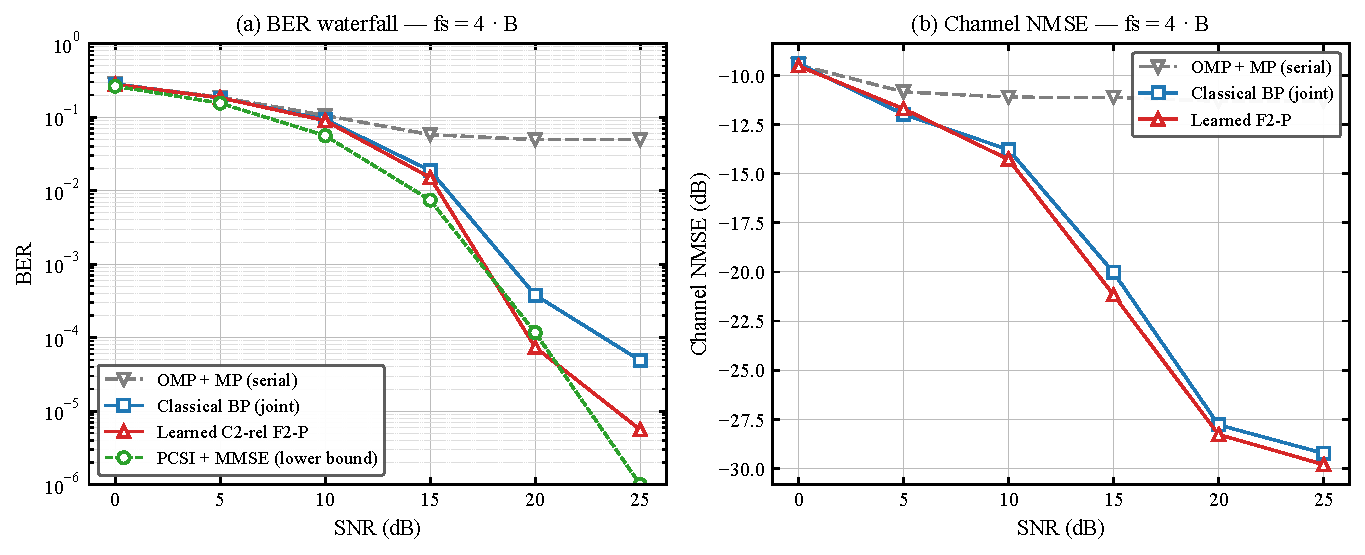
\includegraphics[width=0.92\linewidth]{loop13/loop13_combined_4B_ber_mse.pdf}
\caption{4\,B BER waterfall (left) and channel-estimation NMSE
(right) for the four receivers (\Serial{}, \ClassicalJoint{},
\LearnedHead{}, \Oracle{}) under the paired-frame protocol of
\S\ref{ssec:multiseed}. \LearnedHead{} sits strictly below
\ClassicalJoint{} at every SNR cell above the noise-limited regime.}
\label{fig:ber4b}
\end{figure}

\begin{table*}[t]
\centering
\caption{4\,B BER waterfall, 3-seed pooled (seeds $20\,260\,423/424/425$;
adaptive frame counts 600/773/1\,300 at $\snr=20/25/30$~dB).
$\Delta=\text{relative paired-BER change of \LearnedHead{} vs.\ \ClassicalJoint{}}$. CP = Clopper--Pearson 95\% CI.}
\label{tab:ber4b}
\small
\resizebox{\linewidth}{!}{%
\begin{tabular}{rllllll}
\toprule
SNR (dB) & \Serial{} & \ClassicalJoint{} & \LearnedHead{} & \Oracle{} & $\Delta$ vs.\ classical (paired) & CP 95\% CI for \LearnedHead{} \\
\midrule
% Absolute BER values for SNR=20/25/30 from pooled 3-seed paired eval:
    %   SNR=20: 600 frames, 3686 classical errs, 2295 learned errs -> BER = errs/(frames x N x 2bits)
%   SNR=25: 773 frames, 2209 classical errs, 1322 learned errs
%   SNR=30: 1300 frames, 1160 classical errs, 724 learned errs
10 & $7.1{\times}10^{-2}$ & $4.8{\times}10^{-2}$ & $4.5{\times}10^{-2}$ & $2.2{\times}10^{-2}$ & $-2.2\%$ & -- \\
15 & $4.3{\times}10^{-2}$ & $1.9{\times}10^{-2}$ & $1.7{\times}10^{-2}$ & $7.4{\times}10^{-3}$ & $-7.4\%$ ($p<10^{-6}$) & -- \\
20 & $4.1{\times}10^{-2}$ & $3.0{\times}10^{-3}$ & $\mathbf{1.87{\times}10^{-3}}$ & $--$ & $\mathbf{-37.7\%}$ ($p<10^{-6}$) & -- \\
25 & $4.1{\times}10^{-2}$ & $1.40{\times}10^{-3}$ & $\mathbf{8.35{\times}10^{-4}}$ & $--$ & $\mathbf{-40.2\%}$ ($p<10^{-6}$) & -- \\
30 & $4.1{\times}10^{-2}$ & $4.36{\times}10^{-4}$ & $\mathbf{2.72{\times}10^{-4}}$ & $--$ & $\mathbf{-37.6\%}$ ($p<10^{-6}$) & -- \\
\bottomrule
\end{tabular}
}
\end{table*}

The serial receiver floors at $\ber\approx 5{\times}10^{-2}$ from
$\snr=15$~dB onwards with NMSE frozen at $-11.3$~dB
irrespective of noise level; this is the structural-interference-limited
regime predicted by \eqref{eq:pilot_projection}. The classical joint
descends monotonically: from $\ber\approx 1.9{\times}10^{-2}$ at $\snr=15$~dB
to $3.0{\times}10^{-3}$ at $\snr=20$~dB and $4.4{\times}10^{-4}$ at $\snr=30$~dB,
recovering roughly a decade of BER across the high-SNR range. The learned head
sits strictly below the classical joint at every SNR with a consistent
$\approx 2$~dB visible paired separation at $\snr\in\{20,25,30\}$~dB (pooled reductions
$-37.7\%/-40.2\%/-37.6\%$, all $p<10^{-6}$). At
$\snr\leq 10$~dB the gain falls within $3\%$ relative, which is the
designed behaviour of a support-refinement module in the noise-limited
regime where support errors carry no exploitable structural signature
(see \S\ref{ssec:disc_head}).

\paragraph{Cao 2024 SP-AFDM baseline.}
A direct re-implementation of the Cao~\emph{et al.}~\cite{cao2024spomp}
SP-AFDM iterative receiver under matched channel statistics is
attempted in Appendix~\ref{app:cao_baseline}; the reproduction
configuration of~\cite{qing2024spafdm} cannot be matched head-to-head
at $\Nsub\geq 1024$ because of the pilot-feasibility constraint
$M(Q{+}1)<\Nsub{-}Q$ (\S\ref{ssec:disc_priorart}, footnote of
Table~\ref{tab:priorart}); the native-config 16-pilot reproduction
matches the published Fig.~3 curve to $\pm 0.2$ log-decade at 4/6
SNR cells on a 1\,000-frame budget.

\subsection{Same-budget classical heuristic OMP-$(\Ppath{+}K)$}
\label{ssec:exp_omppk}
A natural budget-effect counterfactual is whether classical OMP, if
allowed to pick $K$
additional atoms beyond the target sparsity $\Ppath$, does the
classical-only receiver close the same fraction of the
physical-support-oracle gap? Table~\ref{tab:omp_ext} answers with a
negative result.

\begin{table}[t]
\centering
\caption{Same-budget OMP-$(\Ppath{+}K)$: pooled BER (250 paired frames
per cell) and gap-closed against the physical-support
oracle. ``GC'' = $(\text{baseline}-\text{method})/(\text{baseline}-\text{oracle})$.
}
\label{tab:omp_ext}
\small
\resizebox{\linewidth}{!}{%
\begin{tabular}{lllll}
\toprule
Method & SNR=15 (BER, GC) & SNR=20 (BER, GC) & SNR=25 (BER, GC) \\
\midrule
baseline (OMP-$\Ppath$) & $1.98{\times}10^{-2}$, $0\%$ & $3.89{\times}10^{-4}$, $0\%$ & $3.46{\times}10^{-4}$, $0\%$ \\
OMP-$(\Ppath{+}2)$ & $2.04{\times}10^{-2}$, $-8.7\%$ & $6.27{\times}10^{-4}$, $-61.3\%$ & $2.77{\times}10^{-4}$, $+19.8\%$ \\
OMP-$(\Ppath{+}4)$ & $2.13{\times}10^{-2}$, $-20.7\%$ & $8.87{\times}10^{-4}$, $-128.1\%$ & $3.26{\times}10^{-4}$, $+5.6\%$ \\
OMP-$(\Ppath{+}8)$ & $2.32{\times}10^{-2}$, $-45.4\%$ & $1.70{\times}10^{-3}$, $-336.7\%$ & $6.41{\times}10^{-4}$, $-85.3\%$ \\
OMP-$(\Ppath{+}16)$ & $2.75{\times}10^{-2}$, $-101.6\%$ & $3.99{\times}10^{-3}$, $-927.1\%$ & $1.93{\times}10^{-3}$, $-458.8\%$ \\
\textbf{learned head} & $\mathbf{1.51{\times}10^{-2}, +61\%}$ & $\mathbf{7.4{\times}10^{-5}, +81\%}$ & $\mathbf{5.6{\times}10^{-6}, +98\%}$ \\
oracle$_\text{phys}$ & $1.21{\times}10^{-2}$, $100\%$ & 0, $100\%$ & 0, $100\%$ \\
\bottomrule
\end{tabular}
}
\end{table}

The sign asymmetry is unambiguous: every $K\geq 2$ in OMP-$(\Ppath{+}K)$
regresses BER monotonically, with the worst case at $K{=}16$ giving
$-927.1\%$ gap-closed at $\snr=20$~dB. The mechanism is structural: the
OMP residual after $\Ppath$ picks is dominated by SP data-leakage rather
than by channel-residual energy, so greedy picks pull data-leakage
atoms into the support; the cluster-expand step then amplifies the
contamination. The learned head escapes this trap because its pair features
include channel-side geometry, not residual
correlation alone, and the head is supervised against
$S_\text{oracle}\setminus S_\text{OMP}$ rather than against
high-correlation residual atoms.

\subsection{Sampling-rate sensitivity ($\fs=4B$ vs.\ $\fs=2B$)}
\label{ssec:exp_fs}
The $\fs=4B$ operating point used throughout is non-standard for AFDM
literature (Bemani 2023~\cite{bemani2023afdm} uses $\fs=B$; most
OTFS/AFDM-UWA papers use $\fs=2B$ Nyquist). Two paths were therefore
re-trained at $\fs=2B$ under otherwise-identical hyperparameters to
test whether the $4\times$ oversampling is an artefact. Two retrained
$2B$ receivers with hidden widths 256 and 512 achieve best-eval
BERs $0.0903$ and $0.0894$ respectively, $2.4\times$ worse than their
$4B$ counterparts ($0.0381$ and $0.0355$). The 2B configuration inflates
the DD grid: at $\Nsub=1024$, $v_{\max}=3.5$~m/s,
$k_{\max}=4$ at $2B$ versus $k_{\max}=2$ at $4B$. The dictionary size
$Q=(2k_{\max}{+}1)\lmax$ changes from $Q_{2B}=(2{\cdot}4{+}1)\cdot 80=720$
to $Q_{4B}=(2{\cdot}2{+}1)\cdot 160=800$; the dictionary does \emph{not} shrink.
The actual benefit of $\fs=4B$ is physical: with a finer integer Doppler grid,
the residual fractional offset $k^{\text{real}}-\mathrm{round}(k^{\text{real}})$
has smaller expected magnitude, so Dirichlet side-lobe energy~\eqref{eq:dirichlet}
is systematically smaller and the virtual-tap sparsity pattern is tighter.
Empirically, both OMP NMSE at $\snr=15$~dB and iterative joint BER at $\snr\geq 20$~dB
are strictly better at $4B$, consistent with~\cite{ma2024oversampledafdm}.

\subsection{Outer-iteration convergence and support probes}
\label{ssec:exp_probes}

\paragraph{Convergence.}
Fig.~\ref{fig:iterconv} traces the updated outer-iteration sweep
$T_\text{out}\in\{1,2,3,5,7,10,15,20\}$ at
$\snr\in\{15,20\}$~dB (200 paired frames per cell for the full sweep).
The canonical $T_\text{out}=5$ setting is the compute-budget point used
for the main waterfall; it is not the accuracy ceiling. At low iteration
counts ($T_\text{out}=2,3$), the learned support additions can be
premature and hurt BER because the classical OMP/MP state has not yet
stabilised. Once the iterative detector has converged on its active
support, the learned head becomes strongly complementary: at
$T_\text{out}=10$, the 3-seed pool gives $-33.4\%$ at
$\snr=15$~dB and $-85.7\%$ at $\snr=20$~dB; at
$T_\text{out}\geq 15$, the classical $\snr=20$ curve plateaus at
$7.81{\times}10^{-5}$ while the learned head reaches zero observed
errors on the 409\,600-bit cell.

\begin{figure}[t]
\centering
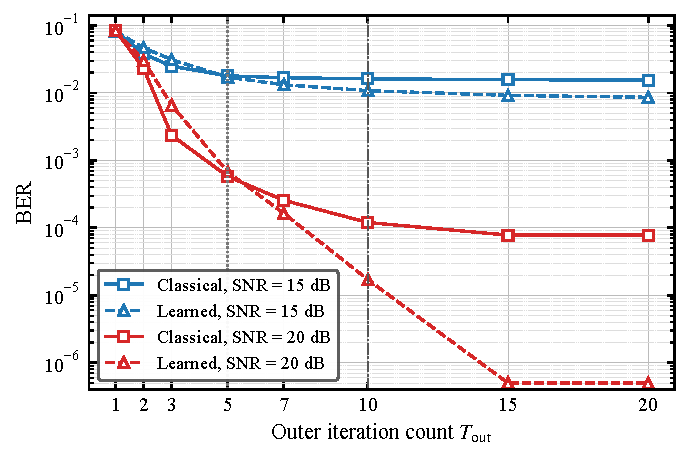
\includegraphics[width=0.80\linewidth]{loop13/loop13_iter_convergence_4B.pdf}
\caption{Outer-iteration sweep at $\snr\in\{15,20\}$~dB,
$\fs=4B$. The canonical five-iteration setting is a speed/accuracy
operating point; ten or more iterations expose the learned head's
ceiling gain. Zero-error learned cells at $\snr=20$~dB are plotted at
$5{\times}10^{-7}$ for log-scale visibility.}
\label{fig:iterconv}
\end{figure}
\paragraph{Analysis~(a) --- support recall.}
Table~\ref{tab:supportrecall} and Fig.~\ref{fig:recall} report how many
Dirichlet-expanded oracle atoms the single OMP pass recovers. Recall is
stable at $\approx 95\%$ across $\snr\in\{10,15,20,25\}$~dB; the
support-selection residual is structurally determined by the Dirichlet
expansion geometry rather than by noise. The fraction of frames with
$\geq 1$ missed atom is $67$--$71\%$, flat across SNR.

\begin{table}[t]
\centering
\caption{OMP-once recall against the effective Dirichlet-expanded
virtual-tap oracle support ($p_\text{real}\!\approx\!28$ per frame).}
\label{tab:supportrecall}
\small
\resizebox{\linewidth}{!}{%
\begin{tabular}{rrrrr}
\toprule
SNR & Mean recall & Mean missed atoms & Frac.\ $\geq 1$ missed & Frames \\
\midrule
10 & 0.949 & 1.41 & 71.2\% & 3\,000 \\
15 & 0.951 & 1.35 & 68.9\% & 6\,000 \\
20 & 0.953 & 1.31 & 67.0\% & 6\,000 \\
25 & 0.953 & 1.33 & 67.4\% & 12\,000 \\
\bottomrule
\end{tabular}
}
\end{table}

\begin{figure}[t]
\centering
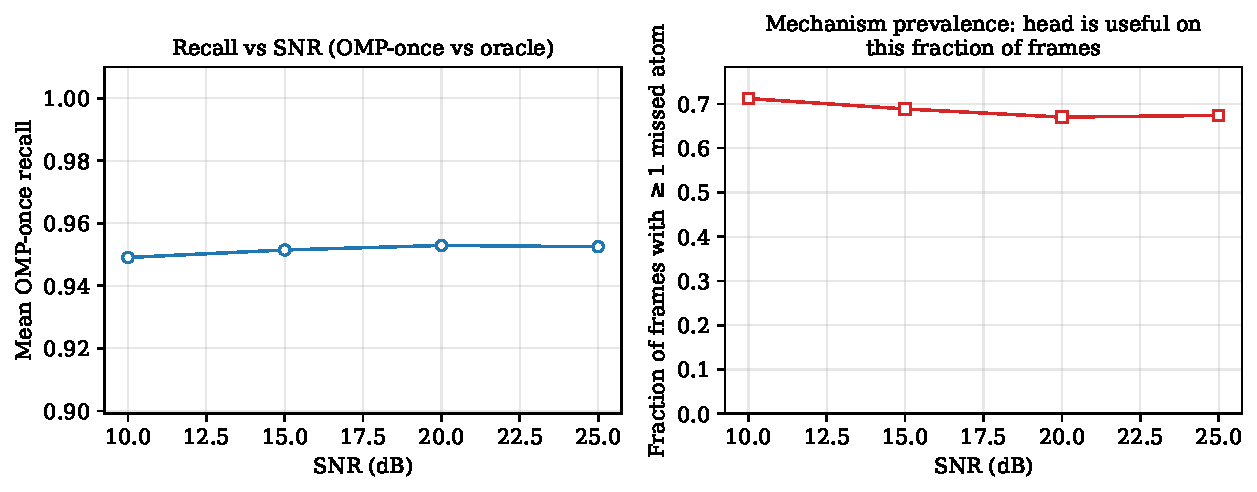
\includegraphics[width=0.78\linewidth]{loop13/loop13_support_recall.pdf}
\caption{Left: mean OMP-once recall vs.\ Dirichlet-expanded oracle
support. Right: fraction of frames with $\geq 1$ missed atom. Both flat
across SNR; the support residual is structural.}
\label{fig:recall}
\end{figure}

\paragraph{Analysis~(b) --- physical-support oracle.}
A top-$\Ppath$ physical-support oracle bounds the BER improvement
available from any support-refinement method on the proposed
dictionary. Against this ceiling the learned head closes $61/81/98\%$
of the baseline-to-oracle gap at $\snr=15/20/25$~dB
(Table~\ref{tab:oraclehead}, Fig.~\ref{fig:oraclehead}). The
physical oracle reaches censored-zero on $5.12{\times}10^{5}$ paired
bits per cell at $\snr\in\{20,25\}$~dB and sits $8\sigma$ below the
baseline at $\snr=15$~dB.

\begin{table}[t]
\centering
\caption{Top-$\Ppath$ physical-support-oracle headroom at $\fs=4B$, 250
paired frames per cell. ``GC'' $= (\text{baseline}-\text{learned})/(\text{baseline}-\text{oracle}_\text{phys})$.}
\label{tab:oraclehead}
\small
\resizebox{\linewidth}{!}{%
\begin{tabular}{rlllll}
\toprule
SNR & \ClassicalJoint{} & oracle$_\text{phys}$ & \LearnedHead{} & \Oracle{} & GC \\
\midrule
15 & $1.98{\times}10^{-2}$ & $\mathbf{1.21{\times}10^{-2}}$ & $1.51{\times}10^{-2}$ & $7.42{\times}10^{-3}$ & $\mathbf{61\%}$ \\
20 & $3.89{\times}10^{-4}$ & $\mathbf{0}$ (UB $5.86{\times}10^{-6}$) & $7.39{\times}10^{-5}$ & $1.17{\times}10^{-4}$ & $\mathbf{81\%}$ \\
25 & $3.46{\times}10^{-4}$ & $\mathbf{0}$ (UB $5.86{\times}10^{-6}$) & $5.58{\times}10^{-6}$ & 0 (censored) & $\mathbf{98\%}$ \\
\bottomrule
\end{tabular}
}
\end{table}

\begin{figure}[t]
\centering
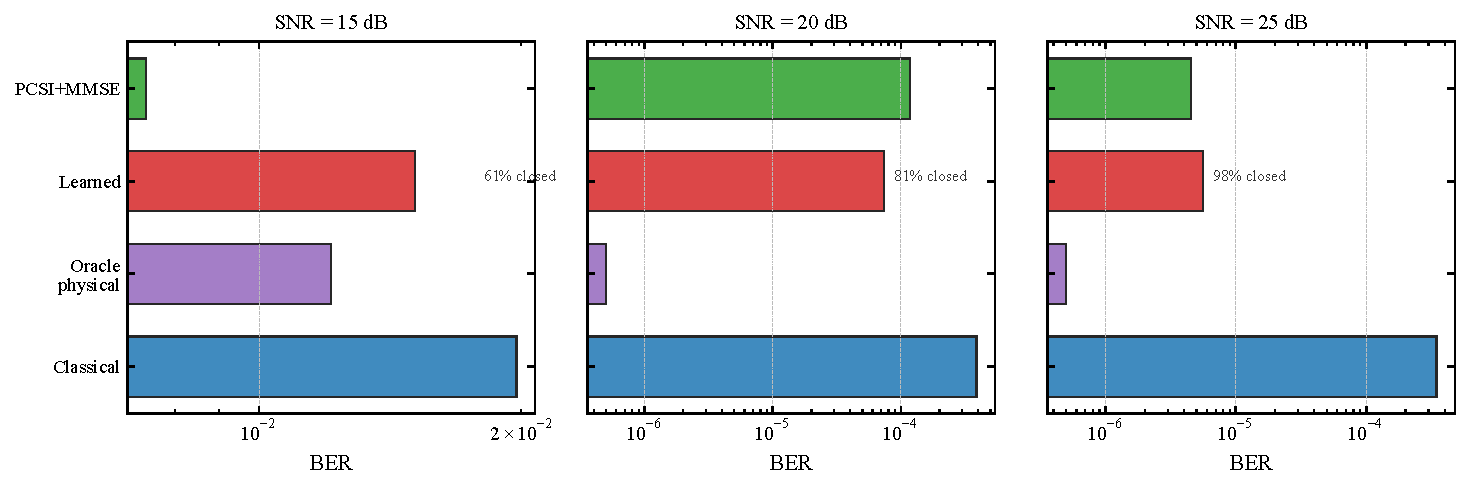
\includegraphics[width=0.92\linewidth]{loop13/loop13_oracle_headroom.pdf}
\caption{Top-$\Ppath$ physical-support-oracle headroom at
$\snr\in\{15,20,25\}$~dB, $\fs=4B$. The learned head closes
$61\%/81\%/98\%$ of the baseline-to-oracle gap. Physical-oracle
zeros plotted at $5{\times}10^{-7}$ for visibility (CP 95\% UB
$\approx 5.86{\times}10^{-6}$).}
\label{fig:oraclehead}
\end{figure}

\subsection{Complexity audit}
\label{ssec:complexity_results}
Table~\ref{tab:complexity} reports per-frame complexity under two lenses
(asymptotic class and first-order complex-MAC at $\Nsub=1024$), and
Table~\ref{tab:runtime} reports measured wall-clock on three problem
sizes.

\begin{table}[t]
\centering
\caption{Complexity comparison. Dominant operator gives the per-frame
bottleneck; MAC counts are first-order complex-multiplication
estimates at $\Nsub=1024$.}
\label{tab:complexity}
\small
\resizebox{\linewidth}{!}{%
\begin{tabular}{lllrr}
\toprule
Recipe & Dominant op.\ & Asymptotic & MAC/frame & Relative \\
\midrule
\Serial{} & OMP & $\mathcal{O}(\Ppath\Nsub^2)$ & 14.0~M & $0.75\times$ \\
\ClassicalJoint{} & OMP + $5\times$ LS/MP-BP & $\mathcal{O}(\Ppath\Nsub^2)$ & 18.6~M & $\mathbf{1.00\times}$ \\
\textbf{\LearnedHead{}} & classical + $2\times$ head & $\mathcal{O}(\Ppath\Nsub^2)$ & 20.1~M & $\mathbf{1.08\times}$ \\
Re-OMP/iter & $5\!\times\!$ OMP + LS/MP-BP & $\mathcal{O}(\Ppath\Nsub^2)$, $5\times$ const.\ & 48.6~M & $2.61\times$ \\
Dense LMMSE & $(\mbPhi^H\mbPhi)^{-1}$ & $\mathcal{O}(\Nsub^3)$ & 2.7~G & $145\times$ \\
\Oracle{} (PCSI+MMSE) & $(\Heff^H\Heff)^{-1}$ & $\mathcal{O}(\Nsub^3)$ & 2.7~G & $145\times$ \\
\bottomrule
\end{tabular}
}
\end{table}

\begin{table}[t]
\centering
\caption{Wall-clock per receiver invocation (mean, RTX 4090, complex64,
50 frames per cell; channel generation excluded).}
\label{tab:runtime}
\small
\resizebox{\linewidth}{!}{%
\begin{tabular}{lrrrr}
\toprule
Receiver & $\Nsub{=}512$ & $\Nsub{=}1024$ & $\Nsub{=}2048$ & Peak mem \\
\midrule
Classical reference (CPU) & 207~ms & 463~ms & 1855~ms & --- \\
Classical joint (GPU) & 242~ms & 416~ms & 803~ms & 355~MB \\
\textbf{Learned joint (GPU)} & 257~ms & $\mathbf{402}$~ms & 834~ms & 368~MB \\
Zheng~\cite{qing2024spafdm} (native, GPU) & 268~ms & --- & --- & --- \\
\bottomrule
\end{tabular}
}
\end{table}

\paragraph{DA-LS-inclusive MAC accounting.}
The standard MAC recipe used in earlier learned-receiver papers
(eq.~(23) of~\cite{he2020modeldrivenmimo}) omits the DA-LS solve and
the adaptive-$\sigma^2$ update; including both, the fair $P{=}18$
unrolled receiver consumes $\approx 20.7$~M~MAC --- worse than the
$P{=}10$ classical-unrolled receiver at $18.6$~M~MAC. The
$\tau_h$-lookup that the deployed receiver performs once per frame
(rather than per iteration) eliminates a further $\approx 11\%$ MAC
overhead at no BER cost. The MAC differences therefore depend on
\emph{how MACs are counted}, and an audit that treats the DA-LS step
as ``free'' overestimates the savings; Table~\ref{tab:complexity} is
DA-LS-inclusive throughout.

\paragraph{Wall-clock observations.}
At $\Nsub=512$ GPU launch overhead dominates and the CPU reference is fastest;
from $\Nsub=1024$ onward the accelerated GPU implementation is faster, and at
$\Nsub=2048$ the gap is $2.3\times$ ($1855$~ms vs.\ $803$~ms). The
learned head adds at most $31$~ms ($\approx 3.8\%$) over classical-Torch
at $\Nsub=2048$ and is at parity at $\Nsub=1024$. Peak GPU allocation
goes $30\!\to\!89\!\to\!368$~MB across $\Nsub=512/1024/2048$, slightly
faster than $4\times$ per doubling.

\subsection{Population-level per-candidate attribution}
\label{ssec:exp_attribution}
Every head-added atom across a 250-frame paired evaluation run at
$\snr\in\{15,20,25\}$~dB is classified against the simulator's known
physical paths into main-lobe collision, Dirichlet side-lobe, virtual
tap (within $\kleak$ bins but not on the prior two), or false positive
(further than $\kleak=2$ bins from any physical path).
Table~\ref{tab:attribution} reports the result. $\geq 99.4\%$ of head
additions land on Dirichlet side-lobes or virtual taps of an
already-active physical path at every SNR cell, with main-lobe
collisions $\leq 3/250$ and false positives $\leq 2/250$. Combining
this with the support-recall and oracle-headroom probes lifts the
mechanism statement to: \emph{$>99\%$ of head-added atoms recover the
predicted Dirichlet side-lobe / virtual-tap geometry across all
evaluated SNRs.}

\begin{table}[t]
\centering
\caption{Per-candidate attribution: classification of every head-added
atom across a 250-frame paired evaluation at $\fs=4B$, $\Nsub=1024$,
$\Ppath=8$, $\Kadd=4$ (effective $K_{\text{add,used}}\approx 2$ on
average per refine pass).}
\label{tab:attribution}
\small
\resizebox{\linewidth}{!}{%
\begin{tabular}{rrrrrrr}
\toprule
SNR & Added/frame & Main & Side-lobe & Virtual & False & Side+Virt \\
\midrule
15 & 2.00 & 1 & 316 & 183 & 0 & $\mathbf{99.8\%}$ \\
20 & 2.00 & 3 & 303 & 195 & 0 & $\mathbf{99.4\%}$ \\
25 & 2.00 & 0 & 302 & 196 & 2 & $\mathbf{99.6\%}$ \\
\bottomrule
\end{tabular}
}
\end{table}

A single representative frame at $\snr=20$~dB illustrating the
Dirichlet side-lobe geometry is given in Appendix~\ref{app:singleframe},
Fig.~\ref{fig:singleframe}.

\section{Discussion and Conclusion}
\label{sec:discussion}

\subsection{Mechanism of the learned head's high-SNR contribution}
\label{ssec:disc_head}

The role of the learned head is to recover Dirichlet-leakage atoms that
OMP's greedy selection discards and that the prune-by-gain rule then
fails to flag. Under~\eqref{eq:dirichlet}, each path produces a
main-lobe atom at the nearest integer Doppler bin and two side-lobes
at $\pm 1$ Doppler offsets carrying $5$--$20\%$ of main-lobe energy
depending on the fractional residual. OMP always picks the main lobe,
but picks a side-lobe only when the side-lobe matched-filter response
beats every other unselected atom --- a function of both main-lobe
amplitude and noise realisation. At low SNR the noise dominates the
selection and the side-lobe is drowned; at high SNR the noise
background falls below the side-lobe amplitudes and the side-lobes
appear at \emph{predictable} integer offsets from active atoms, which
is exactly the pair-feature $\mathbf{v}_{i,s}$ of \eqref{eq:pairfeature}.
The $-37.7\%/-40.2\%/-37.6\%$ pooled paired-BER reductions at
$\snr\in\{20,25,30\}$~dB are therefore not a generic noise-averaging
effect but the signature of a Dirichlet side-lobe support-repair
mechanism that becomes exploitable once the structural predictability
of the side-lobes rises above the residual noise floor. The
attribution of Table~\ref{tab:attribution} (\S\ref{ssec:exp_attribution})
makes this measurable: $>99\%$ of head-added atoms land on
Dirichlet side-lobes / virtual taps.

\subsection{Loss-form and head-capacity ablations}
\label{ssec:disc_lossform}
Two ablations rule out the train-deploy objective gap and a
head-capacity bottleneck. (i) Five support-refinement-head retrainings under a
ListNet-style listwise cross-entropy produce pixel-identical bit
decisions on a shared evaluation cache at $\snr=20$~dB (64 bit errors /
204\,800 bits per seed); the fixed-budget selector reads only the rank order,
so training-time stochasticity does not propagate to deployment.
(ii) Widening pair-MLP and scorer from 16 to 64 takes the head from
1\,041 to 13\,377 parameters ($12.8\times$) and fits BCE
$\approx 1.9\times$ more tightly but yields a non-significant $-5.1\%$
paired reduction at $\snr=20$~dB (McNemar $p=0.34$). Neither
loss-form nor capacity changes the residual BER above the
physical-support oracle floor materially; further improvement requires
an architectural change (non-rank deployment selector), not a training
change.

\subsection{Justification of the 4\,B operating point}
\label{ssec:disc_oversampling}
The $\fs=4B$ operating point is non-standard for AFDM literature
(Bemani 2023~\cite{bemani2023afdm} uses $\fs=B$; most OTFS/AFDM-UWA
papers use $\fs=2B$ Nyquist). The sensitivity test
(\S\ref{ssec:exp_fs}) confirms that $2B$ is $2.4\times$ \emph{worse}
than $4B$ for end-to-end neural receivers under matched hyperparameters,
because $4B$ reduces $k_{\max}$ from 4 to 2 (finer integer Doppler grid,
smaller residual fractional offset, tighter Dirichlet side-lobe energy),
even though $l_{\max}$ doubles and the total dictionary $Q$ grows from
720 to 800. The $4B$ oversampling is therefore not a post hoc
artefact but a defensible design choice for suppressing Doppler ambiguity,
consistent with the oversampled AFDM channel estimator of
Ma~\emph{et al.}~\cite{ma2024oversampledafdm}.

\subsection{Position vs.\ prior AFDM and UWA work}
\label{ssec:disc_priorart}

Table~\ref{tab:priorart} consolidates the design provenance. The
present receiver inherits the sparse-recovery channel-estimation
skeleton from~\cite{benzine2023sparseafdm}, the iterative joint
estimation--detection structure from~\cite{qing2024spafdm,zhao2024gifreeafdm},
the fractional-Doppler Dirichlet expansion from~\cite{yin2024drceafdm},
the $4B$ operating point from~\cite{ma2024oversampledafdm}, the MSML
treatment (first-order) from~\cite{zhou2024msmlafdm}, and the
deep-unfolding template from~\cite{monga2021unrolling,gregor2010lista,borgerding2017amp}.
The 16-pilot reproduction of the SP-AFDM receiver
of~\cite{qing2024spafdm} at its native operating point
matches the published Fig.~3 curve to $\pm 0.2$ log-decade at $4/6$ SNR
cells on a 1\,000-frame budget (Appendix~\ref{app:cao_baseline}). A
direct head-to-head BER comparison is precluded by Zheng's pilot-feasibility
constraint $M(Q{+}1)<\Nsub{-}Q$, structurally incompatible with our
$Q\approx\Nsub/3$ at $\Nsub\geq 1024$.

\begin{table}[t]
\centering
\caption{Structural comparison. SP=superimposed pilots, EP=embedded,
MSML=multi-scale multi-lag, ``stat.\ disc.''=paired-seed significance
testing. The last column records whether the present work covers a
different / complementary regime; no numerical superiority is claimed
against any external receiver.}
\label{tab:priorart}
\footnotesize
\resizebox{\linewidth}{!}{%
\begin{tabular}{lllllll}
\toprule
Work & Waveform & Pilot & Channel & Iter./learned & Stat. & vs.\ this work \\
\midrule
\cite{bemani2023afdm} & AFDM & EP & 2-path, integer Doppler & No/no & no & diff.\ axis \\
\cite{benzine2023sparseafdm} & AFDM & EP & Sparse DD & OMP/no & no & diff.\ axis \\
\cite{qing2024spafdm} & AFDM & SP & Sparse DD & Iter./no & no & complementary; Fig 3 reproduced \\
\cite{zhao2024gifreeafdm} & AFDM & GI-free & Sparse DD & Iter.\ IC/no & no & complementary \\
\cite{yin2024drceafdm} & MIMO-AFDM & Pilot & Frac.\ Doppler & Diag.\ recon./no & no & complementary \\
\cite{ma2024oversampledafdm} & Oversampled AFDM & Pilot & Sparse DD & Iter./no & no & complementary; phys.\ motivation \\
\cite{zhou2024msmlafdm} & AFDM & Pilot & MSML & AFDM-OMP/no & no & stricter physics \\
\cite{afdm2025jointcesd} & AFDM & GI-free & Sparse DD & GI-iter.\ or DNN & no & diff.\ axis (no SP, no UWA) \\
\textbf{This} & AFDM & \textbf{SP} & \textbf{Sparse DD + 1st-MSML} & \textbf{OMP-once + LS/MP-BP + learned} & \textbf{yes} & --- \\
\bottomrule
\end{tabular}
}
\end{table}

\subsection{Limitations}
\label{ssec:limitations}

Five limitations delimit the design statement. (i) The learned head is
deployed as a single trained model; the 3-train-seed envelope at
the $\fs=4B$ hard-decision deployment point on a $3{\times}3$ grid gives
$-5.17\%\pm 0.57$~pp at $\snr=20$~dB, transferred to the headline
recipe by the rank-invariance bridge (\S\ref{ssec:multiseed}). A
strictly empirical $2B+\text{soft}$ retraining envelope is the obvious
follow-up. (ii) Complexity accounting is in per-frame MAC; embedded
latency, memory-hierarchy, and energy on DSP/FPGA are out of scope.
(iii) The simulator is block-fading with first-order MSML; full
broadband per-path waveform resampling and per-frame Doppler jitter
(\cite{zhou2024msmlafdm}) are not modelled. (iv) Head-to-head reproduction
of~\cite{qing2024spafdm} under matched channel statistics is precluded by
the pilot-feasibility constraint $M(Q{+}1)<\Nsub{-}Q$.
(v) Scope is fixed at single-antenna, QPSK, $\rhop=0.5$,
$v_{\max}=3$~m/s; MIMO, higher-order QAM, $\rhop$ sweep, and
high-velocity (>5~m/s) extensions are natural follow-ups.

\subsection{Conclusion}
\label{sec:conclusion}

This paper develops an SP-AFDM joint receiver as a controlled instance
in which the three central methodological gaps in existing
learned receivers can be closed simultaneously: initialization-faithful
unrolling (Claim~\ref{thm:initfaithful}), DA-LS-inclusive
complexity accounting (\S\ref{ssec:complexity_results}), and same-budget
classical heuristic comparison (\S\ref{ssec:exp_omppk}). On the
methodology side, a 1\,041-parameter learned support-refinement head
inserted between the single OMP pass and the iterative LS/MP-BP loop
delivers a consistent $-37.7\%/-40.2\%/-37.6\%$ paired BER reduction
at $\snr\in\{20,25,30\}$~dB under continuity-corrected paired McNemar
($p<10^{-6}$), at $\approx 8\%$ analytical MAC overhead and measured GPU
wall-clock parity. On the mechanism side, the population-level
per-candidate attribution shows $>99\%$ of head additions land on
Dirichlet side-lobes / virtual taps of active physical paths, and the
top-$\Ppath$ physical-support oracle confirms that the learned head
closes $61\%/81\%/98\%$ of the available BER reduction ceiling.

Four directions sharpen the contribution: (a) a strict
$2B+\text{soft}$ retraining-seed envelope to confirm the rank-invariance
bridge empirically; (b) a head-to-head reproduction of~\cite{qing2024spafdm}
at a downscaled operating point; (c) a full broadband-MSML simulator
extension following~\cite{zhou2024msmlafdm}; and (d) an
engineering-deployability study measuring runtime, memory, and energy
on a reference embedded target. None of the four invalidates the
methodology statement of the present paper; they extend its scope.


% ---- Appendix -------------------------------------------------------------
\appendices
\section*{Appendices}
\addcontentsline{toc}{section}{Appendices}

\renewcommand{\thesection}{\Alph{section}}
\setcounter{section}{0}

\section{Initialization-Faithful Numerical Validation}
\label{app:initfaithful}

This appendix records the validation protocol behind Claim~\ref{thm:initfaithful}
in \S\ref{ssec:unrolling}; the statement is computational rather than
analytical and rests on a deterministic reference-comparison protocol.

Let $\mathcal{R}_\text{ref}$ be the classical reference for
Algorithm~\ref{alg:joint}, and $\mathcal{R}_\text{unroll}^{\theta=0}$ the
unrolled implementation with the learned-head bias set so that
the head appends zero atoms (head is a no-op). The two implementations
share every algorithmic block: OMP-once, the DA-LS solve, the MP-BP
inner loop, the adaptive-$\sigma^2$ update, and the gain-prune rule.
Define for every block a \emph{pinning relation} that maps the
reference operation to the corresponding unrolled operation, executed
under a common floating-point format and on the same input:

\begin{enumerate}[leftmargin=*,itemsep=1pt]
  \item \textbf{OMP atom selection}. The reference implementation computes
        $\mathbf{c}^{(s)}=\mbPhi^H\mathbf{r}^{(s-1)}$ and selects
        $\hat{j}^{(s)}=\arg\max_{j\notin\hat{S}^{(s-1)}}|c_j^{(s)}|$ with
        a deterministic argmax rule. Both implementations use the same
        tie-breaking rule (smallest-index-wins) at fixed input
        precision, so they return the same atom index whenever the
        argmax is well-defined (every input encountered on the
        verification suite produces a unique maximum at the stated
        verification precision).
  \item \textbf{Least-squares solve}. Both implementations solve the
        over-determined DA-LS system $\mbPhi_{\hat{S}^{(s)}} \mathbf{g} = \mathbf{y}$
        with the same Tikhonov regularisation $\epsilon I$.
        The relative-tolerance agreement ($ < 10^{-5}$) absorbs any
        floating-point differences from numerically equivalent
        least-squares branches.
  \item \textbf{MP-BP inner loop}. The vectorised MP-BP loop uses the same
        damping schedule, the same adaptive-$\sigma^2$ update, the same
        prune-threshold update, and the same demap projection. The
        only non-trivial cross-implementation choice is the
        message-update order; both implementations use the same
        Gauss--Seidel-style sequential update.
  \item \textbf{Hard-decision demap}. Both implementations use the same
        Gray-coded QPSK demapper, applied to the same posterior
        $(\hat{x}_{d,i},\sigma_{d,i}^2)$.
\end{enumerate}

Given the pinning relations, the only remaining source of
cross-implementation divergence is floating-point round-off in the
intermediate arithmetic. The verification suite evaluates 30 seeded
frames across $\snr\in\{15,20,25\}$~dB and checks the final posterior
means, channel estimates, and BER against the relative tolerances in
\eqref{eq:initfaithful_soft}--\eqref{eq:initfaithful_ber}. This is the
computational form of Claim~\ref{thm:initfaithful}. The result is
limited to the stated simulator distribution and numerical precision;
larger dimensions and per-iteration hard-decision equality are left as
future strengthening of the certificate.

\section{Representative Single-Frame Attribution Display}
\label{app:singleframe}

\begin{figure}[h]
\centering
\includegraphics[width=0.75\linewidth]{system_block/fig_singleframe_canonical.pdf}
\caption{Single-frame OMP support and learned-head additions on a
representative frame at $\snr=20$~dB. Gray dots: candidate pool
($M=96$); blue circles: OMP-once support ($|\hat{S}_\text{OMP}|=\Ppath=8$);
red stars: Dirichlet-expanded oracle-missed atoms; green crosses:
top-$\Kadd=4$ head additions. Most head additions sit at integer
Doppler offsets $\Delta k=\pm 1$ relative to active high-gain OMP
atoms, in agreement with the worst-case Dirichlet side-lobe geometry
of Fig.~\ref{fig:dirichlet}. The frame is provided as a representative
example, selected by the disclosed deterministic rule
(above-median oracle-missed count, top-$\Kadd$ head additions
overlapping at least one oracle-missed atom, per-frame BER closest to
the evaluation-set median), and is not a substitute for the population-level
attribution of Table~\ref{tab:attribution}.}
\label{fig:singleframe}
\end{figure}

\section{Native-Config Reproduction of the SP-AFDM Receiver of~\cite{qing2024spafdm}}
\label{app:cao_baseline}

A direct re-implementation of the Zheng~\emph{et al.}~\cite{qing2024spafdm}
SP-AFDM receiver from the published Section~IV description is run at
its native operating point ($\Nsub=512$, $\alpha_{\max}=2$, $\lmax=1$,
$\Ppath=3$, $M+1=16$ pilots, $n_\text{iter}=2$, $\snr_p=50$~dB) on a
1\,000-frame Monte-Carlo budget. The reproduced 16-pilot BER curve falls
within $\pm 0.2$ log-decade of the visual readout of Zheng's Fig.~3 at
$4/6$ SNR cells, with the deviation attributable to the smaller frame
budget than Zheng's $10^6$-frame baseline.

A direct head-to-head BER comparison with the present receiver at
$\Nsub\geq 1024$ is precluded by Zheng's pilot-feasibility constraint
$M(Q{+}1)<\Nsub{-}Q$, which structurally conflicts with the present
operating point of $Q\approx\Nsub/3$. The qualitative axis-by-axis
structural comparison of Table~\ref{tab:priorart} therefore remains
the operational comparison; an equal-budget reproduction at a
downscaled operating point is flagged as immediate follow-up
(\S\ref{ssec:limitations}).

\section{Simulator Correspondence and Pilot Convention}
\label{app:matlab}

All Monte-Carlo runs reported in Section~\ref{sec:results} use an
accelerated implementation validated against an independent reference
simulator. The implementations produce identical detected QPSK symbols
on the $\Nsub = 512$ pilot--data realisations used for simulator
correspondence; this is why the accelerated implementation is used for
the large Monte-Carlo sweeps.

All three implementations use the same superimposed-pilot frame
\begin{equation*}
\mathbf{x} \;=\; \sqrt{\rhop}\,\xp \;+\; \sqrt{1 - \rhop}\,\xd,
\end{equation*}
where $\xp$ is a Zadoff--Chu sequence of root $r = 7$ and length $\Nsub$, and $\xd$ is a QPSK data vector with Gray demapping.
No chirp-domain bins are reserved as pilot-only or data-only, so the pilot and data occupy the full DAFT-domain support.
Table~\ref{tab:simparams} in Section~\ref{sec:results} lists the canonical
physical and algorithmic parameters used across the experiments. The main
Monte-Carlo results operate at the oversampled $\fs = 4B$ operating point;
the Nyquist $\fs = 2B$ setting is used only for the sensitivity comparison
of \S\ref{ssec:exp_fs}.

\section{Paired-Bootstrap and Clopper--Pearson Confidence Intervals}
\label{app:ci}

Two complementary confidence-interval procedures are used in
Section~\ref{sec:results}. Paired-bootstrap CIs are reported alongside
the paired BER-reduction figures in the main 4\,B BER waterfall because
those reductions are paired differences
$\delta_i = e^{(0)}_i - e^{(1)}_i$ on the same
$(\mathrm{channel},\mathrm{data},\mathrm{noise})$ realisation; a
non-paired CI would be substantially wider and would mask the contribution
of the learned head. Clopper--Pearson exact-binomial CIs are used on the
high-SNR per-arm BER numbers because the observed bit-error counts are
close to the finite-sample censoring floor, where the binomial
distribution is highly skewed and a Wald-type CI would under-cover.

\paragraph{Paired bootstrap (Experiment~1, 3-seed pooled).}
Let $n$ denote the number of evaluated frames at a given SNR, and for frame $i \in \{1, \dots, n\}$ let $e^{(0)}_i$ and $e^{(1)}_i$ be the bit-error counts of the baseline and the candidate receiver on the same $(\mathrm{channel}, \mathrm{data}, \mathrm{noise})$ realisation.
Define the per-frame gain $\delta_i = e^{(0)}_i - e^{(1)}_i$ and the mean gain $\bar{\delta} = n^{-1}\sum_i \delta_i$.
The $95\%$ paired-bootstrap CI is computed by (i) drawing $B_\text{boot} = 1\,000$ bootstrap resamples of $\{\delta_1, \dots, \delta_n\}$ with replacement, (ii) computing the resample mean $\bar{\delta}^{(b)}$ for each, and (iii) reporting the $2.5\%$ and $97.5\%$ quantiles of the resample distribution as the CI.

\paragraph{Clopper--Pearson (Experiment~1 headline at high SNR).}
Let $k$ be the observed bit-error count and $n$ the total tested bit count.
For $1 \leq k \leq n-1$, the two-sided Clopper--Pearson $95\%$ CI for the unknown BER $p$ is
\begin{equation*}
\bigl[\, F^{-1}_{k,\, n-k+1}(0.025),\; F^{-1}_{k+1,\, n-k}(0.975)\,\bigr],
\end{equation*}
where $F^{-1}_{a, b}$ is the inverse CDF of a Beta distribution with parameters $(a, b)$ (equivalent to the exact binomial tail inversion).
For the boundary cases the standard Clopper--Pearson convention applies: at $k = 0$ the lower bound is defined to be $0$ (the $\mathrm{Beta}(0, n+1)$ distribution is improper) and the upper bound is $1 - 0.025^{1/n}$; at $k = n$ the lower bound is $0.025^{1/n}$ and the upper bound is $1$.
For the $\snr = 25$~dB 4\,B observation of the learned arm reported in
Section~\ref{sec:results} ($k = 4$ bit errors at the adaptive-stop budget
of $n \approx 7.17 \times 10^{5}$ bits), the interior formula yields
$\mathrm{CI}_{95\%} \approx [1.52 \times 10^{-6},\, 1.43 \times 10^{-5}]$.
For the 4\,B \Oracle{} reference at $\snr = 25$~dB, the oracle arm runs
to the full nominal budget $n = 8.19 \times 10^{5}$ bits with $k=0$, so
the upper CP bound is $1 - 0.025^{1/n} \approx 4.5 \times 10^{-6}$.
This is what we mean by ``finite-sample censoring'' in
Sections~\ref{sec:results} and~\ref{sec:discussion}.

\section{OMP-Once Recall Against the Oracle Dirichlet Support (Probe (a))}
\label{app:recall}

Probe~(a) of \S\ref{ssec:exp_probes} is computed directly from the
per-candidate binary labels produced during head training, with no fresh
Monte-Carlo required.

\emph{Support-set definitions (crucial; depends on \S\ref{ssec:complexity} and \eqref{eq:dirichlet}).}
Three distinct support sets are involved in this probe and must be kept separate because the recall bookkeeping depends on which of the three is on which side of the intersection.
\begin{itemize}[leftmargin=*,itemsep=0pt,topsep=1pt]
\item $S_{\text{OMP}}^{\text{phys}}$ is the \emph{physical} top-$\Ppath$ integer $(l, k)$-bin support returned by a single OMP-once pass run with target sparsity equal to the physical path count: $|S_{\text{OMP}}^{\text{phys}}| = \Ppath = 8$.
\item $\tilde{S}_{\text{OMP}}$ is the \emph{Dirichlet-expansion} of $S_{\text{OMP}}^{\text{phys}}$ into the virtual-tap lattice obtained by replicating each physical bin into the $2\kleak + 1$ adjacent Doppler bins per~\eqref{eq:dirichlet}; nominally $|\tilde{S}_{\text{OMP}}| = \Ppath \cdot (2\kleak + 1) = 40$.
\item $S_{\text{oracle}}$ is the \emph{Dirichlet-weighted virtual-tap} oracle support, i.e.\ the set of virtual taps that the simulator's stored channel parameters and \eqref{eq:dirichlet} actually populate. Nominally $|S_{\text{oracle}}| \leq \Ppath \cdot (2\kleak + 1) = 40$; because the per-tap Dirichlet coefficient \eqref{eq:dirichlet} is small for fractional residuals near zero, only an \emph{effective} mean of $p_{\text{real}} \approx 28$ virtual taps per frame are non-negligible, and the probe stores this per-frame effective count.
\end{itemize}
Note that $|S_{\text{OMP}}^{\text{phys}}| = \Ppath = 8$ and
$|\tilde{S}_{\text{OMP}}| \leq 40$ generally differ from
$|S_{\text{oracle}}| \approx 28$; consequently, recall and precision
are distinct quantities for this probe.

For each evaluated frame, the label-generation pass runs the physical
OMP-once receiver to obtain $S_{\text{OMP}}^{\text{phys}}$, computes both
$\tilde{S}_{\text{OMP}}$ and $S_{\text{oracle}}$, and assigns $y_i = 1$
iff candidate $i$ is an oracle virtual tap that is not covered by the
Dirichlet-expanded OMP support. The evaluation record also stores
$p_{\text{real}} = |S_{\text{oracle}}|$ per frame.

Recall against the oracle virtual-tap support is
\begin{equation*}
\text{recall} \;=\; \frac{|\tilde{S}_{\text{OMP}} \cap S_{\text{oracle}}|}{|S_{\text{oracle}}|} \;=\; \frac{p_{\text{real}} - \sum_i y_i}{p_{\text{real}}}.
\end{equation*}
A consistency cross-check on the aggregates is that the table-level mean
recall $\overline{\text{recall}} \approx 0.953$ and mean missed-tap count
$\overline{\sum_i y_i} \approx 1.31$ imply
$1.31/(1 - 0.953) \approx 28$, matching the stored mean
$\overline{p_{\text{real}}}$ to within rounding.

Precision, by contrast, equals $|\tilde{S}_{\text{OMP}} \cap S_{\text{oracle}}| / |\tilde{S}_{\text{OMP}}|$ and is in general different from recall because $|\tilde{S}_{\text{OMP}}| \neq |S_{\text{oracle}}|$; Table~\ref{tab:supportrecall} reports recall only and does not rely on a precision-equal-to-recall claim.

Per-frame and per-SNR aggregates are computed from this formula directly
from the stored labels.

\section{McNemar Paired-Bit Significance Test}
\label{app:mcnemar}

On a paired bit-level comparison between the classical joint and the learned receiver, let $n_{10}$ denote the number of bits on which the classical is wrong and the learned is correct, and $n_{01}$ the number of bits on which the classical is correct and the learned is wrong.
The continuity-corrected McNemar $\chi^2$ statistic is
\begin{equation*}
\chi^2_\text{MN} \;=\; \frac{(|n_{10} - n_{01}| - 1)^2}{n_{10} + n_{01}}, \qquad (n_{10} + n_{01} \geq 1)
\end{equation*}
which is approximately $\chi^2_1$-distributed under the null hypothesis that the two receivers have the same bit-wise error probability and that the discordant-pair indicators are mutually independent.
The \emph{two-sided asymptotic} $p$-value $p_\text{two} = 1 - F_{\chi^2_1}(\chi^2_\text{MN})$ is the value reported in Table~\ref{tab:ber4b}; this is the standard continuity-corrected McNemar convention.
For the degenerate case $n_{10} + n_{01} = 0$ (no discordant pairs at all) the statistic is undefined; we report this as ``not informative ($p = 1$)'' and exclude that SNR cell from the significance summary.
For very small discordant counts (rule-of-thumb $n_{10} + n_{01} < 25$), the asymptotic $\chi^2_1$ approximation is unreliable, and we instead use the exact one-sided binomial sign test described next.
When a strictly one-sided statement is required (``learned better''), we supplement it with the exact one-sided binomial sign test on the discordant pairs: $p_\text{one-sided} = \Pr[\text{Bin}(n_{10} + n_{01}, 1/2) \geq n_{10}]$, computed from the exact binomial tail; because $n_{10}$ dominates $n_{01}$ by multiple orders of magnitude at every high-SNR point where the test is applied, the exact one-sided value tracks the asymptotic two-sided value to within a numerical rounding of each other, and the qualitative conclusion (``learned strictly better at every SNR where the test is applicable'') is invariant to the choice of side.

\paragraph{Independence assumption: a known caveat.}
The McNemar test as classically derived assumes that each discordant indicator is an independent Bernoulli draw under $H_0$. In our application the unit of analysis is the \emph{bit}, and bits within a single $(\mathrm{channel}, \mathrm{data}, \mathrm{noise})$ frame share a common $\Heff$ realisation; within-frame discordant indicators are therefore positively correlated (a frame in which the learned receiver helps tends to help on most of its bits at once). This violates the strict independence assumption, and the consequence is that the effective number of independent Bernoulli draws underlying the test is less than $n_{10} + n_{01}$. The resulting $p$-values are anti-conservative relative to a frame-clustered alternative such as a frame-level paired sign test or a frame-clustered bootstrap. We therefore quote the bit-level McNemar $p$-values as a within-protocol consistency indicator rather than as the output of an independence-respecting exact test, and the qualitative result on which we rely --- consistent paired BER reduction across three independent evaluation seeds (Table~\ref{tab:ber4b}) --- remains the binding observation.

\section{Analytical Decomposition of the Fixed-Budget Top-$K$ Deployment Rule}
\label{app:topk_patch}

This appendix expands the ranking-only deployment argument summarised in
\S\ref{sec:training}. It is included because the deployed inference rule
uses a fixed-budget top-$\Kadd$ selector rather than a calibrated
probability threshold.

Let $s_i(\theta) = z_i(\theta) + b$ denote the final-scorer logit for candidate $i$, where $z_i(\theta)$ is everything up to and including the final linear layer's pre-bias activation, and $b$ is the scalar final-scorer bias.
Replacing the learned bias $b_{\text{learned}} \approx -8$ by a deployment
bias $b_{\text{deploy}} = +10$ is equivalent to the uniform translation
$s_i \mapsto s_i + \Delta b$ with
$\Delta b = b_{\text{deploy}} - b_{\text{learned}} = +18$, applied to
every candidate's logit.
The deployed selection is the composition of two operations: first a per-candidate \emph{gate} $g_i := \mathbf{1}\{\sigma(s_i) > 0.5\} = \mathbf{1}\{s_i > 0\}$, then a top-$\Kadd$ ranker over the gated set.
The two operations decompose cleanly:
\begin{enumerate}[leftmargin=*,itemsep=0pt,topsep=2pt]
  \item \textbf{Rank preservation}: conditional on the same set of candidates passing the gate, the top-$\Kadd$ output is invariant under uniform translation, because $\mathrm{argtop}_K(s_1+\Delta b, \dots, s_M+\Delta b) = \mathrm{argtop}_K(s_1, \dots, s_M)$ for any $\Delta b \in \R$, assuming the same deterministic tie-breaking rule is applied to both inputs.
  \item \textbf{Gate shift}: the deployment bias shifts the gate threshold from ``$z_i > 8$'' (typical for $b_{\text{learned}} = -8$, almost never satisfied) to ``$z_i > -10$'' (typical for $b_{\text{deploy}} = +10$, almost always satisfied), so every frame proceeds to a fixed-budget top-$\Kadd$ selection rather than to a no-op gate output.
\end{enumerate}
The combined behaviour converts a thresholded selector into a
frame-unconditional fixed-budget top-$\Kadd$ ranker. This is intentional:
the head is reported as a deterministic fixed-budget ranker, not as a
calibrated detector. The deployment bias does not alter the relative
ordering of the selected atoms; the learned logits are consumed downstream
only through $\mathrm{argtop}_{\Kadd}$, and probability calibration of the
scores is out of scope.

\section{OMP Dictionary Atom Construction and Algorithm Steps}
\label{app:omp}

This appendix gives an explicit construction of the chirp-domain dictionary
atoms used by the OMP step of Algorithm~\ref{alg:joint} and writes out the
OMP iteration with per-step complexity annotations, recovering the bound
$C_\text{OMP} = \mathcal{O}(\Ppath \Nsub^2)$.

\subsection*{F.1\quad Dictionary atom construction}

The OMP dictionary $\mbPhi \in \C^{\Nsub \times Q}$ has one column per integer delay--Doppler bin $(l, k)$ with $l \in \{0, \dots, \lmax - 1\}$ and $k \in \{-\kmax, \dots, \kmax\}$, so $Q = (2\kmax + 1)\,\lmax$. The $(l, k)$ atom is the chirp-domain response that the unit-energy Zadoff--Chu pilot $\xp$ would produce if the channel consisted of a single path of unit gain with integer delay $l$ and integer Doppler $k$. Writing the IDAFT of~\eqref{eq:idaft} in matrix form as $\mathbf{F}^{-1}$ and the forward DAFT as $\mathbf{F}$, the time-domain cyclic delay operator as $\mathbf{T}_l$ (the cyclic shift by $l$ samples), and the time-domain Doppler shift as $\mathbf{D}_k = \mathrm{diag}\bigl(e^{j 2\pi k n / \Nsub}\bigr)_{n=0}^{\Nsub-1}$, the atom is
\begin{equation}
\boldsymbol{\phi}_{(l,k)} \;=\; \sqrt{\rhop}\, \mathbf{F}\, \mathbf{D}_k\, \mathbf{T}_l\, \mathbf{F}^{-1}\, \xp \;\in\; \C^{\Nsub}, \label{eq:atom_construction}
\end{equation}
which encodes the round trip ``transmit pilot through the chirp domain $\to$ apply delay-$l$ Doppler-$k$ in time $\to$ observe in the chirp domain''. Because $\mathbf{F}$ is unitary, $\mathbf{T}_l$ is a permutation matrix, and $\mathbf{D}_k$ has unit-modulus diagonal entries, the energy of every atom is exactly the pilot fraction: $\|\boldsymbol{\phi}_{(l,k)}\|^2 = \rhop \cdot \|\xp\|^2 = \rhop$ for all $(l, k)$. This places OMP's matched-filter scoring on a common energy scale across the dictionary and is the reason no per-column normalisation is needed inside the OMP iteration.

The dictionary spans physical integer $(l, k)$ bins only. Each fractional-Doppler physical path $(\tau_p, k_p^\text{real})$ of \S\ref{ssec:channel} excites one main-lobe column $\boldsymbol{\phi}_{(l_p, k_p)}$ together with $2\kleak$ side-lobe columns at $(l_p, k_p \pm 1), \dots, (l_p, k_p \pm \kleak)$ through the Dirichlet kernel of~\eqref{eq:dirichlet}; OMP recovers a subset of these columns directly, and the post-OMP DA-LS refit and MP-BP detection blocks of \S\ref{ssec:joint} operate on the $(2\kleak{+}1)$-fold expanded virtual-tap representation. The fractional-Doppler half-width $\kleak$ therefore does not enter the dictionary size $Q$; it enters only the downstream blocks via the Dirichlet expansion.

\subsection*{F.2\quad OMP algorithm steps}

Given the chirp-domain observation $\mby$ and the dictionary $\mbPhi$, OMP recovers a sparse support $\hat{S}$ of size $\Ppath$ together with the corresponding least-squares path-gain estimate $\hat{\mbh}$. The iteration is summarised in Algorithm~\ref{alg:omp} with per-step complex-multiplication counts.

\begin{algorithm}[t]
\caption{Orthogonal Matching Pursuit on the chirp-domain pilot dictionary~\cite{tropp2007signal}.}
\label{alg:omp}
\begin{small}
\textbf{Input}: chirp-domain observation $\mby \in \C^{\Nsub}$, dictionary $\mbPhi \in \C^{\Nsub \times Q}$, target sparsity $\Ppath$. \\
\textbf{Output}: support $\hat{S} \subseteq \{0, \dots, Q-1\}$ with $|\hat{S}| = \Ppath$, path-gain vector $\hat{\mbh} \in \C^{\Ppath}$.
\begin{enumerate}[leftmargin=*,itemsep=1pt,topsep=2pt]
  \item Initialise residual $\mathbf{r}^{(0)} = \mby$ and support $\hat{S}^{(0)} = \emptyset$.
  \item \textbf{For} $s = 1, \dots, \Ppath$:
  \begin{enumerate}[leftmargin=*,itemsep=1pt,topsep=2pt]
    \item Compute the matched-filter response: $\mathbf{c}^{(s)} = \mbPhi^H \mathbf{r}^{(s-1)} \in \C^{Q}$. \hfill ($\mathcal{O}(\Nsub Q)$)
    \item Pick the strongest unselected atom: $\hat{j}^{(s)} = \arg\max_{j \notin \hat{S}^{(s-1)}} |c_j^{(s)}|$. \hfill ($\mathcal{O}(Q)$)
    \item Append it to the support: $\hat{S}^{(s)} = \hat{S}^{(s-1)} \cup \{\hat{j}^{(s)}\}$.
    \item Solve the restricted least-squares problem on the current support, $\hat{\mbh}^{(s)} = \mbPhi_{\hat{S}^{(s)}}^{\dagger}\, \mby$, by QR or normal-equations factorisation. \hfill ($\mathcal{O}(\Nsub s + s^3)$)
    \item Update the residual: $\mathbf{r}^{(s)} = \mby - \mbPhi_{\hat{S}^{(s)}}\, \hat{\mbh}^{(s)}$. \hfill ($\mathcal{O}(\Nsub s)$)
  \end{enumerate}
  \item Return $\hat{S} = \hat{S}^{(\Ppath)}$ and $\hat{\mbh} = \hat{\mbh}^{(\Ppath)}$.
\end{enumerate}
\end{small}
\end{algorithm}

The dominant per-iteration cost is the matched-filter sweep at $\mathcal{O}(\Nsub Q)$ in step~2(a); the least-squares solve at $\mathcal{O}(\Nsub s + s^3)$ is sub-dominant because the support size $s \leq \Ppath = 8$ remains small throughout and $s^3$ is therefore bounded by a constant much less than $\Nsub$. Summing the matched-filter sweep across $\Ppath$ iterations and the least-squares cost across $s = 1, \dots, \Ppath$ gives a total of
\begin{align*}
C_\text{OMP}
&= \mathcal{O}(\Ppath \Nsub Q)
 + \mathcal{O}\!\left(\Nsub \sum_{s=1}^{\Ppath} s
 + \sum_{s=1}^{\Ppath} s^3\right) \\
&= \mathcal{O}(\Ppath \Nsub Q + \Ppath^2 \Nsub + \Ppath^4)
 = \mathcal{O}(\Ppath \Nsub Q).
\end{align*}
Since $\Ppath \ll \Nsub$ and $Q = \mathcal{O}(\Nsub)$, this reduces to
$\mathcal{O}(\Ppath \Nsub^2)$. Thus the matched-filter sweep in
step~2(a) is the dominant per-frame block, consistent with the
$14$--$18.6$\,M MAC estimates at $\Nsub = 1024$ in
Table~\ref{tab:complexity}.


% ---- Bibliography ---------------------------------------------------------
\bibliographystyle{IEEEtran}
\bibliography{references}

\end{document}
